\documentclass{sig-alternate-10pt}
%\documentclass[10pt]{sigalternate052015}

\usepackage{amsmath}
\usepackage{amssymb}
\usepackage{xcolor}
\usepackage{url}
\usepackage{times}
\usepackage{xspace}
\usepackage{listings}
\usepackage{code}
\usepackage{algorithm}
\usepackage[noend]{algpseudocode}
\usepackage{tikz}
\usetikzlibrary{arrows,automata,positioning}
\let\proof\relax
\let\endproof\relax
\usepackage{amsthm}
\usepackage{subcaption}
\usepackage{balance}
\usepackage[ampersand]{easylist}
\usepackage{textcomp}
\usepackage{pifont}
\newcommand{\cmark}{\ding{51}}
\newcommand{\xmark}{\ding{55}}

\definecolor{princetonorange}{RGB}{255,143,0}
\definecolor{tmlblue}{RGB}{0,58,120}  % tmlblue == Toronto Maple Leafs Blue!

\newcommand{\todo}[1]{\textcolor{red}{[TODO: #1]}}
\newcommand{\ratul}[1]{\textcolor{blue}{[ratul: #1]}}
\newcommand{\ryan}[1]{\textcolor{green}{[ryan: #1]}}
\newcommand{\dpw}[1]{\textcolor{tmlblue}{[dpw: #1]}}
\newcommand{\todd}[1]{\textcolor{princetonorange}{[todd: #1]}}

\newcommand{\EG}{\emph{e.g.}}
\newcommand{\IE}{\emph{i.e.}}
\newcommand{\ETC}{\emph{etc.}}
\newcommand{\ETAL}{\emph{et al.}}

\newcommand{\sysname}{{\small \sf Methane}\xspace}
\newcommand{\sysnamesec}{{\sf Methane}\xspace}
\newcommand{\propane}{{\small \sf Propane}\xspace}

\newcommand{\para}[1]{\paragraph*{\textbf{#1}}}

\newcommand{\set}[1]{\ensuremath{\{ #1 \} }}
\newcommand{\abs}[1]{\ensuremath{ \lvert #1 \rvert }}

\newcommand{\CD}[1]{\texttt{\small #1}}  % code font
\newcommand{\KW}[1]{\texttt{\small\bfseries{#1}}}

\newcommand{\True}{\CD{true}}
\newcommand{\Define}{\KW{define}}
\newcommand{\Prefer}{\texttt{>>}}
\newcommand{\Path}{\texttt{=>}}
\newcommand{\Link}{\texttt{->}}
\newcommand{\Agg}{\KW{agg}}
\newcommand{\Any}{\KW{any}}
\newcommand{\None}{\KW{drop}}
\newcommand{\In}{\KW{in}}
\newcommand{\Out}{\KW{out}}
\newcommand{\AND}{\texttt{\&}}
\newcommand{\OR}{\texttt{|}}
\newcommand{\NOT}{\texttt{!}}
\newcommand{\Intersect}{\ensuremath{\cap}}
\newcommand{\Union}{\ensuremath{\cup}}

\newcommand{\Exit}{\KW{exit}}
\newcommand{\End}{\KW{end}}
\newcommand{\Start}{\KW{start}}
\newcommand{\Enter}{\KW{enter}}
\newcommand{\Eventually}{\KW{eventually}}
\newcommand{\Already}{\KW{already}}
\newcommand{\Internal}{\KW{internal}}
\newcommand{\Never}{\KW{never}}
\newcommand{\Always}{\KW{always}}
\newcommand{\Through}{\KW{through}}
\newcommand{\LinkKW}{\KW{link}}
\newcommand{\PathKW}{\KW{path}}
\newcommand{\Novalley}{\KW{novalley}}

\renewcommand{\path}[2]{ #1 \mapsto \ensuremath{#2} }

%% grammar
\newcommand{\BNFALT}{\;\;|\;\;}
\newcommand{\hdr}[2]{\flushleft \chdr{\hspace{5mm}#1}{#2}}
\newcommand{\chdr}[2]{\textbf{#1} {#2} \\ \centering}%

\newtheorem{thm}{Theorem}[section]
\newtheorem{defn}{Definition}
\newtheorem{lem}[thm]{Lemma}

\begin{document}

%\CopyrightYear{2016}
%\setcopyright{acmcopyright}
%\conferenceinfo{SIGCOMM '16,}{August 22-26, 2016, Florianopolis , Brazil}
%\isbn{978-1-4503-4193-6/16/08}\acmPrice{\$15.00}
%\doi{http://dx.doi.org/10.1145/2934872.2934909}

\special{papersize=8.5in,11in}
\setlength{\pdfpageheight}{\paperheight}
\setlength{\pdfpagewidth}{\paperwidth}

\title{An Abstraction-based Approach to Network Synthesis}

%\author{Paper \#324, 14 pages}


\author{%
Ryan Beckett\\
  \affaddr{Princeton}
  %\\
  %\email{rbeckett@princeton.edu}
\and
Ratul Mahajan\\
  \affaddr{Microsoft}
  %\\
  %\email{ratul@microsoft.com}
\and
Todd Millstein\\
  \affaddr{UCLA}
  %\affaddr{University of California, Los Angeles}
  %\\
  %\email{todd@cs.ucla.edu}
\and
Jitendra Padhye\\
  \affaddr{Microsoft}
  %\\
  %\email{padhye@microsoft.com}
\and
David Walker\\
  \affaddr{Princeton}
  %\\
  %\email{dpw@princeton.edu}
}

\maketitle


%=====================================================
%
%
%  **Abstract**
%
%
%=====================================================


% Points to make
%
% (1) Lets operators think about topologies/policies at a high-level of abstraction
%     - matches current thinking (e.g., templates)
%
% (2) Promotes a correct-by-construction methodology
%
%     properties that hold over abstract topologies hold over concrete ones
%      - includes correct forwarding behavior
%      - includes reachability (under k-failures)
%
% (3) Enables reusability (e.g., across datacenters) and expansion (e.g., within a datacenter)
%
% (4) lets us scale synthesis to large-scale topologies


\textbf{Abstract---}
We develop techniques for automated reasoning about end-to-end properties of abstract network topologies. We extend a network synthesis tool, \sysname, to allow network operators to write a high-level routing policy over an abstraction of their network topology. From such a specification, \sysname synthesizes a collection router configurations running the distributed Border Gateway Protocol (BGP) that are guaranteed to implement the centralized routing policy for any concrete instantiation of the abstract topology, and for any combination of network failures in the resulting concrete topology.
%
Additionally, properties proven by \sysname over the abstract topology, such as reachability between a source and destination under k-failures, are also guaranteed to hold under any concrete instantiation of the abstract topology.
%
Something something, expandable/incremental networks. Something something scales compilation to large networks. Something something, templates easier to understand.
%These strong guarantees allow operators to reason about the routing behavior of their network at a high-level abstraction, while also generating an efficient low-level implementation.
%
%In addition, operators are able to safely change or expand their network in any way, so long as the new resulting topology also respects the abstraction.
%
We test \sysname out on ... blah blah blah



%=====================================================
%
%
%  **Keywords**
%
%
%=====================================================

%\vspace{0.1in}
%\noindent
%\textbf{CCS Concepts}\\
%$\bullet$ Networks $\rightarrow$ {\em Network control algorithms; Network reliability; Network management;}
%$\bullet$ Software and its engineering $\rightarrow$ {\em Automated static analysis; Domain specific languages}

%\vspace{0.1in}
%\noindent
%\textbf{Keywords}\\
%Propane; Domain-specific Language; BGP; Synthesis; Compilation; Fault Tolerance; Distributed Systems


%=====================================================
%
%
%  **Introduction**
%
%
%=====================================================

\section{Introduction}
\label{sec:introduction}


% Hence, one approach to improving network
% reliability is to develop better languages for network configuration.
% Such languages should be defined at a higher level of abstraction than
% existing configuration languages and provide support built-in support for
% verification of important properties, thereby avoiding entire classes
% of configuration errors automatically.

An important class of networks are the large \emph{structured networks}
commonly deployed in industrial data centers.  These networks run
many critical services and every second of downtime is at best
costly and at worst dangerous.  Unfortunately, it is an enormous 
challenge to keep these complex networks up and
running 24/7~\cite{mahajan+:bgp-misconfiguration,feamster+:rcc,batfish,dc-failure-study}.
Moreover, while hardware faults, rodents, power failures and natural
disasters can all cause significant downtime, studies have shown that
\emph{human error}, which occurs during network configuration or
update, is the single large cause of these
outages~\cite{juniper-study}. 

% These networks often
% host a myriad of services and every second of downtime imposes significant
% financial cost or disruption to consumers.  
Such networks typically have uniform, tree-shaped topologies that involve
hundreds or even thousands of devices.  Since it is not possible for humans
to think about configuring each individual device independently, 
network operators typically classify the devices, assigning them a particular
\emph{role} such as ``top-of-rack switch'' or ``tier-one aggregation switch.''
Each such role is codified as a \emph{configuration template}---a macro 
that may be instantiated with different concrete values to
generate a configuration for each device that plays the role.

Unfortunately, such templates have no particular semantics other than the 
semantics
that one obtains from instantiating a template's parameters.  
\dpw{add blah blah about low-level, assembly language, device by device}
Moreover,
template construction is a manual process:  network engineers do their
best to design templates that will work effectively in the context 
of their particular network topology.  However, there is no support for
validating key properties of an assembly of templates, such as connectivity 
and fault tolerance, 
aside from instantiating the templates and testing.  In addition,
network engineers have no tools to help them design for network
evolution.  For instance, the process of adding new equipment to
expand the capacity of data center may not be compatible with the original
templates, or may cause a trickle-down of changes to be made network-wide.
Each change to a router configuration typically incurs
some risk of temporary instable in a network, so minimizing such changes
is an important design goal.  It is no wonder that a major
network outage, such as the one that grounded all United Air flights
in July 2015~\cite{x}, makes international news every few months.

To combat these problems, we present \sysname, a 
new high-level language designed to 
provide improved support for the configuration of large, structured networks.
\sysname allows network operators to define \emph{abstract network topologies} 
that
classify devices in terms of their roles and how they are connected
to one another.  For instance, a programmer may
define separate roles for ``top-of-rack switch'' and 
``tier-one aggregation switch'' and specify that every top-of-rack switch
is connected to at least two different tier-one aggregation switches,
thereby providing a degree of fault tolerance of one aggregation switch
were to fail.

To specify \emph{routing policy} for such abstract networks,
\sysname borrows notation from the recently-defined \propane
programming language~\cite{propane}.  As such, it is able to
specify the paths that traffic should flow along at a high-level of
abstraction.  However, whereas \propane policies
refer to paths of individual devices, \sysname policies 
refer to paths of abstract roles.  The \sysname compiler compiles such
policies into templates, with one template per role, and these templates
may be instantiated to generate concrete configurations. 

During compilation, the \sysname compiler also analyzes policy with respect to the
abstract topology and guarantees that the configurations will 
faithfully implement the high-level policy on \emph{any} concrete
topology that satisfies the given connectivity invariants.  The compiler
will also optionally perform a second fault tolerance analysis that 
determines the minimum number of link failures required to disconnect
\emph{any} concrete topology that once again satisfies the connectivity
invariants.  

Finally, generated \sysname configurations are designed to
be \emph{evolution-friendly} in the sense that if an operator adds or
removes any single link or device, they are guaranteed that only 
the configurations of adjacent devices need change (for instance, to
activate a port on which the new device is connected).  Doing so
helps minimize network instability as data centers are expanded or devices are
temporarily taken offline for maintenance.

As an aside, a pleasant side effect of this new compiler
infrastructure, designed to make life easier on network operators, is
that for structured networks, it scales substantially better than its
competitor \propane does: as the number of individual devices in a
network grows, the number of distinct roles will often stay constant.
Consequently, the \sysname compiler may be two orders of magnitude
faster than \propane for large structured networks.

To summarize, the central contributions of this paper are:

\begin{enumerate}
\item Design of new topology abstractions involving roles and
connectivity invariants for network programmers.
\item Design of two new algorithms for analyzing routing policy over 
abstract networks: one which
guarantees correct compilation and one which determines fault tolerance 
properties of network policy.  Both algorithms provide guarantees for any 
concrete network satisfying the abstract connectivity invariants.
\item Design of template generation algorithms that support network
evolution.
\item Implementation and evaluation of a \sysname compiler that generates 
configuration templates and is up to two orders of magnitude faster 
than its closest competitor on large networks.
\end{enumerate}


%% Indeed, over the last several years, many researchers have begun to
%% develop such languages~\cite{frenetic,pyretic,pane,nettle,netkat}.
%% However, the bulk of this research has targeted software-defined
%% networks (SDN), a new networking technology that has emerged over the last
%% decade.  Unfortunately, the vast majority of today's networks
%% continue to use traditional networking techology---upgrading to SDN is
%% expensive and technically challenging.

%% In a traditional network, every router runs an independent instance of 
%% a distributed protocol that
%% exchange messages about available routes to destination addresses.  
%% Each router is configured independently, but the overall behavior
%% of the network---the paths from one server to another, for instance---depend
%% upon the 

%=====================================================
%
%
%  **Motivation**
%
%
%=====================================================


\section{Background and Motivation}
\label{sec:motivation}

\begin{figure}[t!]
  \centering
  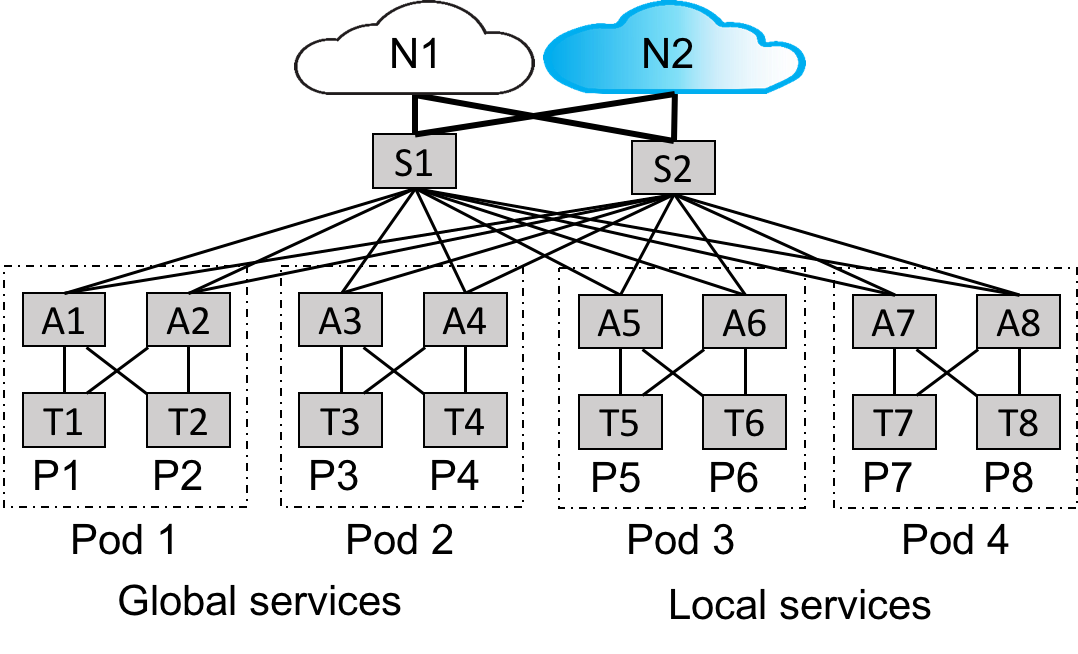
\includegraphics[width=2.5in]{figures/example}
  \caption{An example data center network.}
  \label{fig:example}
  \vspace{-1em}
\end{figure}

\begin{figure}[t!]
  \centering
  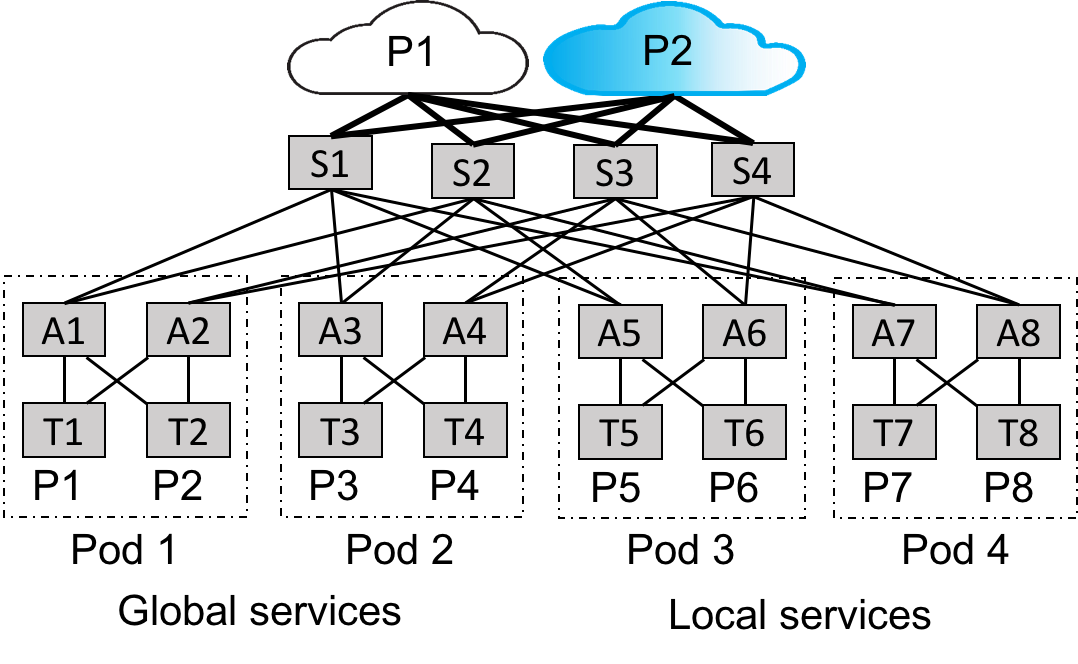
\includegraphics[width=2.5in]{figures/example2}
  \caption{A modified version of the example in Figure~\ref{fig:example}.}
  \label{fig:example2}
  \vspace{-1em}
\end{figure}

\paragraph*{Background}  Traditional routers use 
distributed protocols to exchange messages about available routes. 
One such protocol is the Border Gateway Protocol (BGP).  BGP is the
standard for inter-domain routing (the act of exchanging routing information 
between independently-owned networks) and is also commonly used in
data centers because it allows operators to define relatively flexible
routing policy while also scaling effectively to large networks.
When used within a data center, each router is configured with its own \emph{AS number},
which identifies it.

Each BGP message (also called a \emph{route announcement}) contains a 
\emph{destination prefix}, such as 10.1.1.0/24,\footnote{An address
such as 10.1.1.0 is 32 bits, with each of the four values representing 8 bits.  
A prefix such
as 10.1.1.0/24 denotes the set of addresses that begin with the first
24 bits of 10.1.1.0, \IE, all addresses that begin with 10.1.1.} as well as an
\emph{AS path}, such as XYZ (where each of X, Y and Z would be an AS number).  
Such messages indicate that the set of addresses
denoted by the prefix may be reached by following the path XYZ. 
A BGP message may also contain additional attributes, such as 
\emph{local preference} attribute and one or more
\emph{community values}.

A BGP router may receive messages about the same prefix from several
of its \emph{peers} (\IE, neighbouring routers).  When this occurs,
it processes the messages as follows:
\begin{enumerate}
\item It \emph{filters} (drops) some of the incoming messages based on
any their attributes (AS path, community values, peer it came from, \ETC),
and optionally modifies attributes of the messages it does not drop.
This is usually called the \emph{import} stage.
\item From the remaining messages, it selects the one message it
most \emph{prefers}. Selection is based on a number of criteria, but the
most important is the local preference number: Higher local preferences
are preferred.  Ties are broken by AS path length --- BGP defaults to 
shortest path routing in such cases.
\item Finally, it \emph{exports} the preferred message to selected neighbors,
adding its own AS number to the path and optionally adding or
modifying attributes.
\end{enumerate}
When a BGP router is configured, the user tunes the import and export
stages of the above process, choosing which messages to import, how to
modify them and how to export them.  By modifying the local preferences
on messages in the inport phase, the user determines which messages will
be selected.  This in turn determines how traffic destined for the given
address will be routed.  Keep in mind that if BGP messages to a destination
are propagated in one direction (left-to-right), then traffic will wind
up flowing in the opposite direction (right-to-left).

Rather than export 2$^n$ addresses in the same range, routers will
often perform \emph{route aggregation}, and export a single (32-$n$)-bit
prefix.  During aggregation, whenever an advertisement for 
\emph{any} of the 2$^n$ addresses
reaches the router, the \emph{entire} aggregate prefix will be announced.
While useful for decreasing announcements and avoiding churn, such
aggregation can be dangerous:  If a message for one of the 2$^n$ addresses (X)
reaches the aggregation router, but another one of the addresses (Y)
cannot reach the aggregation router due to a failure then the aggregate
will be announced, possibly drawing traffic to Y, even though Y cannot be
reached.  This is known as an \emph{aggregation-induced black hole}~\cite{route-aggregation}.
Networks should be configured to be sufficiently fault tolerant to minimize
the chances of such black holes.

\paragraph*{An Example}
%We motivate \sysname using an example data center network. Our network, 
Consider the data center network shown in Figure~\ref{fig:example}.  The boxes in the diagram
represent \emph{switches}, and these switches play several different roles:  T[1--8] denote top-of-rack (ToR) switches, A[1--8] denote aggregation switches, and S[1--2] denote spine switches. The spine switches are connected to the
rest of the internet; any traffic to or from the outside world flows through them.  The aggregation switches
serve as a bridge between spine and ToR switches.   Finally, each ToR switch is
connected to a set servers (``a rack''): P[1--8] denote groups of addresses for services hosted in each rack. 
% Such groups are called address {\em prefixes} because they are encoded using the adresses' shared prefix. 

%% We assume that each switch is running an instance of the \emph{Border Gateway Protocol} (BGP), 
%% as is common in large data centers. In this protocol, adjacent switches use BGP to exchange messages
%% with one another concerning the availability of routes to destinations.  A BGP \emph{configuration}
%% (one for each switch) dictates which offered routes a switch will select and how to propagate chosen routes to its 
%% neighbours.\footnote{If this submission is accepted and more space is available in the final version, 
%% we will give a detailed explanation of BGP for the PLDI audience.  Henceforth, we assume knowledge of basic BGP
%% mechanics.}

%Assume that all nodes are running the border gateway protocol (BGP), as is common in large data centers~\cite{x}. \todo{more detail on BGP?}

The intended high-level operator policy for this network is as follows. Internal connectivity should be complete, \IE, all nodes must be able to talk to each other. Services in Pods 1 and 2 should be globally accessible and thus their addresses should be announced externally, but only after aggregating individual prefixes P[1--4] into a single prefix PG. Finally, services in Pods 3 and 4 not should be externally visible and thus their address should not be announced externally.

To correctly configure the policy above, the network engineer's task is to generate low-level configurations for each switch in the network. This implies ensuring, for instance, that all switch interfaces are assigned correct addresses; all routing adjacencies are correctly configured (\EG, T1's configuration includes A1 as neighbor and vice-versa); all switches announce their own addresses (so that they can be reached for management purposes) and the ToRs announce the correct prefixes for their services; all switches  forward the prefix announcements that they should to each neighbor and not forward those that they should not (\EG, the spines should forward prefixes for local services to internal neighbors but not external neighbors); and the spines announce externally only the aggregate global prefix. \dpw{Do we need to explain aggregation here?}

As many have observed before, such configuration tasks are highly challenging. Consequently, configuration errors are the leading cause of network outages~\cite{juniper-study,bgpmon,batfish,propane}.

\paragraph*{Limitations of concrete synthesis}

In response, researchers have developed systems that synthesize low-level device configurations from high-level policy statements~\cite{narain:lisa05,narain+:configassure,dadc,propane}.
%They take network topology and policy as input and output device configurations that are  guaranteed to be correct under all possible failures. Thus, they save the engineers from performing the complex task of breaking down global policies into device configurations.
These systems eliminate entire classes of configuration errors by construction, and, in the case of
Propane~\cite{propane}, guarantee that high-level policy is implemented correctly, even in the presence of 
arbitrary combinations of failures.

However, our conversations with network engineers at two major cloud providers reveal that they have two limitations that discourage adoption.  The first is a mismatch in abstraction. Engineers of large, structured networks tend to think of the network, and to develop management tools, using \emph{roles}, and not individual devices. 
A {\em role} refers to specific functionality and is played by one or more routers. The network in Figure~\ref{fig:example} has five roles: spine, global aggregator, global ToR, local aggregator, and local ToR.  Engineers are naturally reluctant to use a system that does not 
understand roles as a first-order abstraction because they think about 
network policy in terms of roles, and, even more importantly, if they want to debug, analyze or 
understand system output, they will have to consider 
\emph{hundreds} of independent device configurations instead of just
\emph{a handful} of role configurations. Unfortunately, even if two devices play the same role,
there is no guarantee a concrete synthesis system will generate (syntactically) similar configurations,
making vetting system outputs extremely difficult. 

A second limitation is the inability to support network evolution. Networks evolve all the time as nodes and links are added or removed and the addresses of services are changed. A system that supports evolution would ensure that 
small changes in topology require small, local changes in network configurations as opposed to pervasive
changes across many devices.  Engineers want to minimize changes to device configurations because each change runs the risk of poor, transient behavior due to poor router software or routing protocol dynamics~\cite{ratulbgpmisconfigs}.  
%These networks must be highly
%available; it isn't plausible to bring down an entire data center network, or large portions of it, to make
%incremental changes.

Unfortunately, in general, any change in network topology requires re-execution of a
concrete synthesis engine, from scratch,
on the changed topology.  The result may be 
a completely different set of configurations.  However, even if such configurations are
largely semantically similar to existing configurations, they may be syntactically different,
and may cause considerable network disruption when updates are pushed to switches.
For instance, suppose an operator wants to modify the prefix of local ToR T8 in Figure~\ref{fig:example}. To accommodate the modification, Propane, a concrete synthesis tool, will, at a minimum, not only change T8's configuration but also those of the two spines because it uses prefix lists at spines to ensure that local prefixes are not advertised externally.  As we show later, there is a way to design the configurations of this network to avoid spine configuration changes while accommodating ToR prefix (and other) modifications.  Our new 
abstraction-based synthesis framework synthesizes evolution-friendly roles automatically.

%nof the new spine configurations outputted by Propane will not only enable the interfaces that connect to the new aggregators but will also have to update the prefix list filters. A system that supports incremental growth should need only interface configuration changes (not filter changes). It can configure all local ToRs, including the new ones, to attach a tag to their announcements and filter external announcements at the spines based on this tag. Engineers prefer fewer configuration changes because each change runs the risks of poor transient behavior (which synthesis tools do not reason about).


%For instance, suppose the engineers want to add another pod with local services to the network in Figure~\ref{fig:example}. In this network, Propane, a concrete synthesis tool, uses prefix lists at spines to ensure that local prefixes are not advertised externally. To accommodate the expansion, the new spine configurations outputted by Propane will not only enable the interfaces that connect to the new aggregators but will also have to update the prefix list filters. A system that supports incremental growth should need only interface configuration changes (not filter changes). It can configure all local ToRs, including the new ones, to attach a tag to their announcements and filter external announcements at the spines based on this tag. Engineers prefer fewer configuration changes because each change runs the risks of poor transient behavior (which synthesis tools do not reason about).


\paragraph*{Limitations of today's template systems}

To simplify network configuration, and thus reduce errors, the network engineering community is adopting a template-based approach~\cite{hatch,thwack}. Instead of authoring one configuration file per router, engineers author one configuration template per role.\footnote{If a role is played by devices from different vendors, there is one template per role-vendor combination because templates use vendor configuration language.} Templates have parameters for various aspects of the configuration (\EG, interface addresses, neighbor list) and are compiled to device configurations by instantiating the parameters using a database of per-device values.

%Templates provide two key advantages. First, they help eliminate a class of configuration errors that stem from typos and inconsistencies, e.g., using the wrong address for a switch, having inconsistent addresses for the two ends of a link, and failing to configure one side of a routing adjacency.  Second, templates have the potential for re-use when the topology changes while maintaining its basic structure (e.g., adding a new pod to the data center) or multiple networks with similar structures need to be instantiated (e.g., in an organization that runs multiple data centers).

While templates operate at the right level of abstraction, today's template systems have two limitations. The first is that they offer no correctness guarantees. To author correct templates, engineers must break down complex, network-wide routing policy into role templates such that the collective behavior of the configurations generated from the templates correctly implements the desired high-level policy under all failure conditions.  This is a challenging, manual task, with no tools available to support template verification.

As a result, the types of configuration design errors pointed in prior work~\cite{propane} can occur in template design as well. For instance, to keep local prefixes internal the engineer may implement announcement forwarding on spines based on the identity of the neighbor, \IE, do not announce externally anything heard from local aggregators. This implementation is appealing because it does not require changes to spine configurations when ToR prefixes change. But it works correctly only when there are no failures; local prefixes can leak externally when failures disconnect a spine from both aggregators in a local pod. Specifically, when S1 is disconnected from A5 and A6, it may hear about P5 and P6 from A3 and A4 (via A[5--6]->S2->A[3--4]), and it will then announce those prefixes outside (since they no not come from a local aggregator), leading to a policy violation. A possible correct implementation here would be for each spine to block messages headed to external peers from local aggregators {\em and} to reject announcements that have traversed the other spine (\IE, to disallow "valleys," or up-down-up paths).

%Lacking correctness guarantees, engineers use simulations to analyze if templates are correct under a range of failure cases (e.g., combinations of two-link failures), but such analysis is highly expensive for large networks and still does not provide strong guarantees beyond the tested cases.

The second limitation of today's template systems is that, like concrete synthesis tools, they do not support network evolution. One might hope that important network properties such as connectivity and fault tolerance persist when networks evolve in ways consistent with existing roles and templates.  However, existing 
template systems provide no guarantees that seemingly-minor variations of a given topology have similar properties.    
%In theory, templates do not have to be redesigned when the network evolves while keeping its basic structure of roles and their inter-connectivity. In practice, however, it is not guaranteed that templates that work for a given topology also work for seemingly-minor variations of the topology. 

Consider the network in Figure~\ref{fig:example2}, which is similar to Figure~\ref{fig:example}, with the same folded-Clos structure and five roles. One might think that the same templates (with different database entries) can be re-used across topologies. However, that is not necessarily true.  For example,
data centers are often susceptable to a phenomenon called an \emph{aggregation-induced black hole}~\cite{route-aggregation}.  Such black holes occur when a switch announces an aggregate prefix but has no valid path to a more specific prefix within the aggregate, so the black hole will draw traffic, but that traffic will be unable
to reach its destination.
For instance, if a network operator uses templates designed for Figure~\ref{fig:example}, which
disallow valley paths, on Figure~\ref{fig:example2}, they will find that while it takes two link failures to
trigger a black hole in  Figure~\ref{fig:example}, it takes only 1 failure to trigger a black hole in
 Figure~\ref{fig:example2}.   
More specifically, in Figure~\ref{fig:example2}, a blackhole will occur when the link S1--A1 fails; after this failure, S1 has no valley-free path to P[1--2] even though it will continue to get traffic for these prefixes by virtue of announcing the encompassing aggregate PG. In contrast, in Figure~\ref{fig:example}, no such blackhole will occur after a single failure.

Thus, engineers today must reason about the correctness of templates for each topology change (using expensive simulations because current systems do not provide any correctness guarantee by design). Worse, for some changes, they may discover that their old templates will not work anymore and need modifications. ~\dpw{Note: This is going to be true for Methane too.}  This discovery is highly problematic because changing a template will cause a change in the configurations of all the devices that use that template---in many cases, an unacceptable disruption.  When that happens, network operators may abandon templates entirely and revert to hand-crafting configuration files, using localized patches to accommodate evolution. 
Such patches reintroduce the complexity and errors that templates were meant to prevent.


%As an aside, a possible template implementation that works correctly for both networks is: allow valley paths and use an explicit list of local prefixes at spines to decide which announcements should not be forwarded externally.

\begin{figure}
\begin{tabular}{|p{0.6in}|p{0.6in}p{0.7in}p{0.6in}|} 
\hline
& Abstract Roles & Correctness Guarantees & Evolution Support  \\ \hline
Concrete Synthesis & \xmark & \cmark & \xmark \\ \hline
Template Systems & \cmark & \xmark & \xmark \\ \hline
\sysname & \cmark & \cmark & \cmark \\  \hline
\end{tabular}
\caption{Comparing configuration techniques.}
\label{fig:marketing}
\end{figure}


\subsection{\sysnamesec}

As Table~\ref{fig:marketing} shows, \sysname addresses the limitations of both concrete synthesis and current template systems. It operates at the right level of abstraction for network operators, provides strong guarantees about compiled configurations, supports verification of important correctness properties, and supports network evolution. As inputs, \sysname takes a global, network-wide policy (as opposed to a per-device or even per-role policy) and an 
{\em abstract} topology that describes device roles and 
connectivity invariants.  It outputs a template for each role.  Per-device configurations may be generated
from templates by instantiating their parameters with concrete values drawn from the network topology. 
\sysname provides strong guarantees about its templates: 
(1) the configurations generated from them correctly implement the specified policy for {\em any} concrete topology that matches the given abstract topology; and (2) if you add or remove a single node or edge in a way compatible
with the abstract topology, only configurations of adjacent devices ever need to be updated.

The next section introduces \sysname using the example in Figure~\ref{fig:example}, and the following sections provide more detail on how we generate the templates and formally define the correctness guarantees.


%=====================================================
%
%
%  **Methane Overview**
%
%
%=====================================================

\section{Methane overview}
\label{sec:overview}

As we have seen, writing correct network configurations is challenging task. Operators must manually decompose network-wide policies into distributed device configurations, reason about all combinations of network failures, and parameterize configurations to allow for change, ideally in a way that is amenable to incremental change. In this section, we give an overview of the \sysname system, which gives operators a principled way to accomplish all of these tasks.

%\subsection{Concrete Methane}%

%Consider again the datacenter from figure~\ref{fig:example}. To configure the datacenter routing
%policy, we would start by writing the following definition in \sysname:
%%
%\begin{code}
%\Define Routing =
%    \{P1 \Path \End(T1)
%     P2 \Path \End(T2)
%     P3 \Path \End(T3)
%     P4 \Path \End(T4)
%     P5 \Path \End(T5)
%     P6 \Path \End(T6)
%     P7 \Path \End(T7)
%     P8 \Path \End(T8)
%     \True \Path \Exit(Peer1 \Prefer Peer2) \}
%\end{code}
%\noindent%%

%This defines a group of constraints for basic routing behavior. The first line states
%that traffic destined for prefix $P1$ must follow a path that ends up at destination router $T1$.
%A similar constraint is added for each of the prefixes P[2-8]. The final rule matches all other
%prefix destinations and allows traffic to follow a path that leaves the datacenter through either
%of its peers (Peer1 or Peer2) with a preference for leaving through Peer1. The \Prefer symbol indicates
%that traffic should satisfy the constraint on the left whenever possible, and only resort to the backup (right)
%when this is not possible due to failures.%

%Next we can add the locality constraint for prefixes P[5-8]. We do this by adding another group of constraints:
%%
%\begin{code}
%\Define Locality =
%    \{P5 | P6 | P7 | P8 \Path \Always(\In)\}
%\end{code}
%\noindent%%

%The Locality constraint applies to any traffic destined for a local prefix and adds
%the constraint that the traffic must follow a path that matches an internal location
%(\IE, a router inside the datacenter) at each hop of the path. This prevents traffic
%from ever entering from or leaving through an external peer.%

%Finally, for all traffic in the datacenter, we will disallow valley routing. This constraint
%can be captured with the following additions to the policy:
%%
%\begin{code}
%\Define Tor = \{T1,T2,T3,T4,T5,T6,T7,T8\}
%\Define Agg = \{A1,A2,A3,A4,A5,A6,A7,A8\}
%\Define Spn = \{S1,S2\}
%\Define ValleyFree =
%    \{\True \Path \Novalley(Tor,Agg,Spn)\}
%\end{code}
%\noindent%%

%The first three lines define groups of routers. The top of rack (Tor) routers T[1-8], the
%aggregation routers (Agg) A[1-8], and the spine routers (Spn) S[1-2]. The next line
%adds a new constraint that applies to all traffic and ensures that traffic never follows a
%path that forms a valley between any of these three groups (\EG, going from Spn to Agg to Spn again).
%As we will see in section \ryan{reference}, each of these constraints such as the valley free constraint
%are really just syntactic sugar for regular expressions over topology locations.%

%The final policy is declared to as the conjunction of each of these constraints:
%%
%\begin{code}
%\Define Main =
%    Routing &
%    Locality &
%    ValleyFree &
%    \Agg(PG, \In -> \Out)
%\end{code}
%\noindent%
%The last part of the policy declares that we want to perform aggregation for global prefixes
%by summarizing them into the more general prefix PG at the border of the datacenter
%(\IE along any edge starting inside our datacenter and ending outside).%

%From this policy, \sysname can synthesize device-level BGP configurations for every router in
%the network that guarantee correct forwarding behavior under all possible failure combinations.
%Synthesizing configurations for each device from a network-wide specification both simplifies
%network configuration by writing policy in one place rather than dozens and simultaneously prevents
%a large class of errors associated with manual configuration by construction. For example,
%the compiler ensures configurations are always in sync and prevents the operator from having
%to manually consider failure scenarios.


\subsection{Abstract Compilation}

\sysname builds on the Propane network configuration tool, by supporting both synthesis for and reasoning over parameterized classes of topologies and their interactions with user-specified routing policy. 
\sysname takes as input, (1) a topology abstraction in the form of a graph homomorphism annotated with logical constraints about node and edge mutliplicities, and (2) a domain-specific routing policy that consists of a mapping from predicates matching various classes of traffic, to a list of ranked constraints on the paths traffic matching the predicate should prefer to take through the network.

\para{Topology Abstraction}

Consider again the networks from \S\ref{sec:motivation}. Ideally, we would like
to find a suitable topology abstraction that can describe both of the datacenters from figures~\ref{fig:example} and~\ref{fig:example2} as well as any reasonable generalization of these datacenters. \sysname provides several abstraction mechanisms to achieve this goal. 

The first is a role-based abstraction that allows an operator to map routers in the concrete network to ``roles" or routers in the abstract network. Figure~\ref{fig:example3} shows an example of an abstraction for both datacenter networks from \S\ref{sec:motivation}. In particular the concrete networks are abstracted into a new topology with 5 different roles: local tor (TL), global tor (TG), local aggregator (AL), global aggregator (AG), and spine (S). 

More specifically, a network topology is a graph $G$ = ($V, E$), which consists of a set of vertices $V$ and a set of directed edges $E \colon V \times V$. A role-based abstraction is a graph homomorphism from $G$ to an abstract graph $G^A$ = ($V^A$,$E^A$). A graph homorphism $f : G \rightarrow G^A$ is a function that maps each node in the concrete graph to a node in the abstract graph such that, whenever $(u,v) \in E$, then $(f(u),f(v)) \in E^A$. 


\begin{figure}[t!]
  \centering
  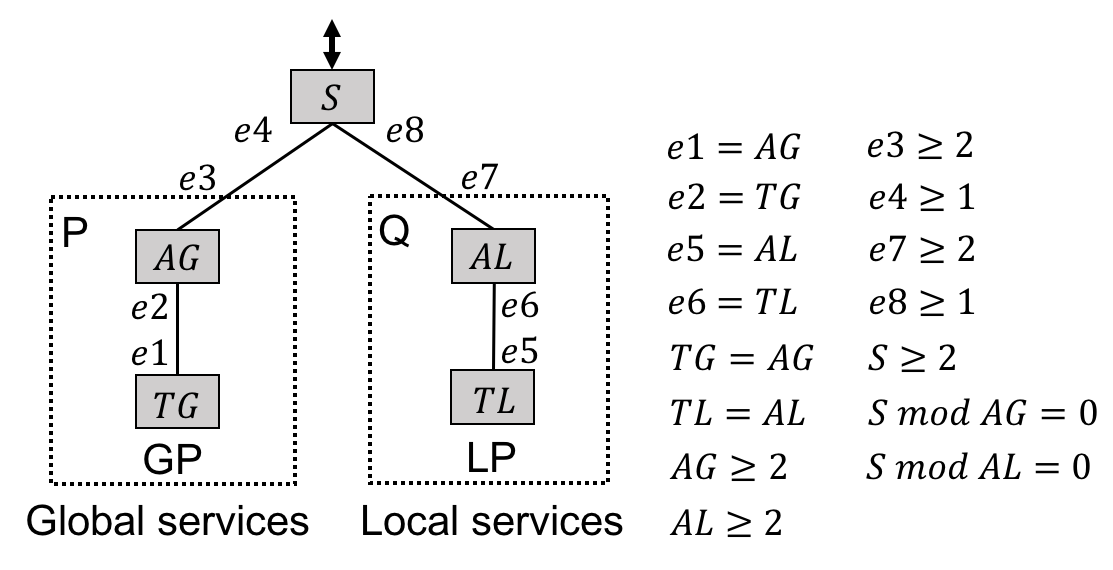
\includegraphics[width=\columnwidth]{figures/example3}
  \caption{Role-based abstraction for the datacenters in Figure~\ref{fig:example}.}
  \label{fig:example3}
  \vspace{-1em}
\end{figure}

The role-based abstraction therefore overapproximates the connectivity of the underlying concrete graphs. Unfortunately this abstraction alone loses a lot of information about the underlying structure of the concrete network. For example, with this abstraction any spine router in a concrete network may or may not be connected to any aggregator router.
%
In order to refine the abstraction to capture more precisely the kinds of concrete networks of interest,
we introduce a notion of node and edge \emph{multiplicities}. Each edge (and node) is labelled
with a symbolic variable (\EG, $e1, e2, \ldots$) that denotes a constraint on the number of nodes/edges
that may appear in any given concrete network. Operators can then capture concrete network invariants by adding constraints on the symbolic variables using logical formula.

For example, in Figure~\ref{fig:example3}, the first two constraints: $e1 = AG$ and $e2 = TG$ declare that, within any pod P, the number of outgoing edges from $TG$ to $AG$ is equal to the number of nodes that map to $AG$. Similarly, the number of outgoing edges from $AG$ to $TG$ is equal to the number of nodes that map to $TG$. These constraints capture the fact that, within any given pod, the global aggregators and tors are in a full mesh. Furthermore, the constraints $TG = AG$ and $TG \geq 2$ ensure that the number of concrete nodes in role $TG$ is always equal to the number of concrete nodes in role $AG$, which is at least 2. Similar constraints also appear for the local aggregators and tors.
%
The constraint $e3 \geq 2$ says that, in each pod, each aggregator node has at least 2 outgoing edges to nodes in the spine role. Symmetrically, the constraint $e4 \geq 1$ says that, for each pod P, each node in the spine role has at least one outgoing edge to a node in the $AG$ role. Again, similar constraints appear for the local aggregator role. Finally, the constraints $S \geq 2$, $(S \mod AG) = 0$, and $(S \mod AL) = 0$ ensure that there are at least 2 routers in the spine role, and that the number of spine routers is always divisible by the number of global and local aggregators.
%
The last two constraints are interesting in that they do not involve a simple inequality. In general operators can write constraints using logical formula for any theory supported by modern SMT solvers. 

All the guarantees provided by \sysname hold for any instantiation of the abstract network. This means that operators can safely expand their network in the future so long as the new network also satisfies these logical constraints.



%Although the concrete \sysname policy can help prevent a number of configuration errors,
%the policy is intricately linked to the actual structure of the concrete network.
%For example, each prefix in the routing constraint is enumerated with its concrete destination
%location, and the definition of the valleyfree constraint depends on the actual routers that
%comprise each tier of the datacenter.
%
%This is unfortunate since any expansion of our datacenter network will require a corresponding
%change to the policy. Furthermore, there is no guarantee that a safe policy can be found
%for the expanded network, and even if one can be found, it may require changes to every
%configuration in the network -- a huge barrier to adoption in practice.

%Abstract \sysname solves this problem in two ways. First, it allows operators to abstract
%the network into a role-based topology and write a routing specification over this abstraction instead.
%Second, it introduces prefix template variables into the language to allow writing policies that are
%parameterized over prefix destination.

\para{Routing Policy}

Next let us see how to configure each of the datacenter networks from \S\ref{sec:motivation} by writing a \sysname routing policy over the new abstract topology. In \sysname, we can capture the basic routing behavior for the datacenters with the following constraints:
%
\begin{code}
\Define Routing =
    \$GP  \Path \End(TG)
    \$LP  \Path \End(TL)
    \True \Path \Exit(Peer1 \Prefer Peer2)
\end{code}
\noindent%

The first line introduces a prefix \emph{template} variable. It says that traffic for each global prefix associated with the template variable \$GP has the constraint that it should follow a path that ends at its corresponding destination router contained in the abstract TG role. The second line does the same thing for all local prefixes. 
%
The final rule matches all other IP prefix destinations and allows traffic to follow a path that leaves the datacenter through either of its peers (Peer1 or Peer2) with a preference for leaving through Peer1. The \Prefer~symbol indicates that traffic should satisfy the constraint on the left whenever possible (\IE, a path exists in the network), and only resort to the backup (right) when this is not possible due to failures.%

Next we can capture the constraint that traffic for local prefixes must stay local to the datacenter.
We do this with the following \sysname constraint:
%
\begin{code}
\Define Locality = 
    \$LP \Path \Always(\In)
\end{code}
\noindent%
%
The Locality constraint applies to any traffic destined for a local prefix described by the \$LP prefix template variable and adds the constraint that the traffic must follow a path that matches an internal location (\IE, a router inside the datacenter) at each hop of the path. This prevents traffic from ever entering from or leaving through an external peer. Finally, we can combine these constraints together as follows:

\begin{code}
Routing & Locality & \Agg(PG, \In -> \Out)
\end{code}
\noindent%

\ryan{we may need to add notransit constraint to make the compilation section simpler}

This tells \sysname to find BGP router configurations that satisfy the conjunction of the Routing and Locality constraints. It also declares an additional constraint that we want to perform prefix summarization (as PG) for global prefixes at the border of the datacenter (\IE, along any edge starting inside our datacenter and ending at a peer outside the datacenter).

When \sysname compiles the above policy, it guarantees that the forwarding behavior of the network will be correct for any concrete instantiation of the abstract network, and for any combination of failures that may occur in the concrete network. Furthermore, \sysname will generate configurations in such a way that, if we want to expand our network, for example by adding or removing a spine routers as in figure~\ref{fig:example2}, then the expansion can be performed by only ever touching device configurations that are adjacent to the change.

\subsection{Abstract Analysis}

Although \sysname can ensure correct forwarding behavior independent of the exact concrete topology or failure scenario, it is often useful to be able to ask "what if" questions about other network properties. For example, an operator may require a certain level fault tolerance between between different collections of routers. Such analysis depends, not only on the network topology, but also on the underlying routing policy, both of which \sysname has access to. To this end, we develop a sound analysis over abstract topologies to answer questions about the number of disjoint paths between pairs of nodes.

Suppose we want to find a worst-case lower bound on the fault tolerance between any global tor and spine router from figure~\ref{fig:example3} for any concrete topology after applying the routing policy. This can be used as a lightweight verification tool to detect certain classes of configuration bugs. For example, since the network is performing prefix summarization at the border of the datacenter, we might introduce a black hole after enough failures occur to disconnect a tor from a spine router.

We develop a disjoint path analysis works in the following way. For each abstract role in the network, we learn invariants about the number of disjoint paths to routers in that role. These invariants contain a sequence of labels followed by a pair of numbers $(i,j)$. For example, the analysis would start with a fact of the form: $S_P S_{TG} (1,1)$. This means that, there is some group of nodes of size 1 in the TG role in some pod P such that any initial node in the TG role has 1 disjoint path to it (and all such paths are edge-disjoint). Since we know that the each node in the TG role is in a full mesh with nodes in the AG role within any given pod, we might infer a fact for AG of the form: $S_P A_{AG}(e1,1)$. This says that any group of nodes of size e1 in the AG role is reachable with at least 1 edge-disjoint path to each such node from any initial node in the TG role.
%
If we run the abstract analysis over the abstract network from figure~\ref{fig:example3} the analysis will learn a fact of the form $A_{S}(1,2)$, which means that any single spine node is reachable via 2 disjoint paths from any initial global tor node \ryan{it will actually be 1, we need to add a constraint on e1}. 

Suppose now that we want to disallow paths with valleys (\IE, paths that go down and then up at some point). Such a constraint can be added to the routing policy in \sysname:
\begin{code}
\Define ValleyFree =
    \True \Path \Novalley(\{TL,TG\},\{AL,AG\},\{S\})
\end{code}
\noindent%

This adds a constraint that applies to all traffic and prevents valleys by defining each level in the datacenter.
Because the abstract analysis is policy sensitive, if we were to run it again with the same abstract topology but the new routing policy, it would only be able to infer that there is a single disjoint path to any given spine router in the worst case. In fact this is exactly the case for the concrete network from figure~\ref{fig:example2}.  

%
%The constraint prevents traffic from over taking a path that traverses
%either [Agg->Tor->Agg] or [Spn->Agg->Spn]. The final policy remains the same as before,
%by combining each of these policies together.
%
%


%=====================================================
%
%
%  **Compilation**
%
%
%=====================================================

\section{Compilation}
\label{sec:compilation}

Configuration synthesis for network configurations is challenging for a number of reasons. First, although \sysname polices specify stable network-wide routing behavior, actual configurations are per-device and run distributed algorithms to compute routes. Thus the compiler must ensure that the result of the distributed computation matches the policy. Furthermore the distributed computation must compute the correct paths under all possible combinations of failures. Second, \sysname must find configurations that work across any valid concrete network topology matching the abstraction provided as input. Finally, \sysname must ensure that the resulting configurations can be evolved incrementally so that local changes to the topology ensure that only local changes to configurations are required to ensure global routing correctness. 

In this section, we formalize the \sysname language and topology abstraction, describe how \sysname synthesizes network configurations over these abstractions, and formalize the guarantees provided by \sysname.

\subsection{Methane Language}

\begin{figure}[t]\small
  \begin{minipage}[t]{\linewidth}
  \vspace*{-1\baselineskip}
  %
  \[ \begin{array}{rclr}
     pol     &::=& p_1, \dots, p_n & \textit{policies} \\
     p       &::=& t \hspace{.3em} \Path \hspace{.3em} r_1 \Prefer \dots \Prefer r_m & \textit{constraints} \\
     t       &::=& \$x & \textit{template variable} \\
         &\BNFALT& d.d.d.d/[d..d] & \textit{prefix test} \\
     r       &::=& l & \textit{location} \\
         &\BNFALT& \emptyset & \textit{empty set} \\
         &\BNFALT& \In & \textit{internal loc} \\
         &\BNFALT& \Out & \textit{external loc} \\
         &\BNFALT& r_1 \cup r_2 & \textit{union} \\
         &\BNFALT& r_1 \cap r_2 & \textit{intersection} \\
         &\BNFALT& r_1 \cdot r_2 & \textit{concatenation} \\
         &\BNFALT& \NOT r & \textit{path negation} \\
         &\BNFALT& r^* & \textit{iteration} \\
  \end{array} \]%

  \end{minipage}
  \vspace{1em}
  \caption{Simplified \sysname syntax.}
  \label{fig:syntax}
  %\vspace{-1em}
\end{figure}%

The syntax introduced in \S\ref{sec:overview} is just syntactic sugar for a core language based on regular expressions. Figure~\ref{fig:syntax} shows a simplified version of the core \sysname syntax that omits some details such as aggregation. The full langauge definition can be found in the appendix. 

A policy has one or more constraints, each of which consists of a test on the type of traffic being matched and a corresponding set of preferred regular expressions describing network paths. Regular expressions are defined over network locations, where each location is either a router inside the operators network, or an external neighbor. There are two special characters \In~ and \Out, which match any internal and external location respectively. There are two types of predicates: a test for a concrete prefix $d.d.d.d/[d..d]$ matches an IP prefix with value $d.d.d.d$ and length in the range $[d..d]$ where metavariable $d$ represents an integer. For example, the IP prefix 148.0.1.0/[24..32] would match traffic destined for IP address 148.0.1.* with a subnet length between 24 and 32 bits. \ryan{this needs to be explained clearer}.

Converting from the high-level syntax from \S\ref{sec:overview} to the core syntax is straightforward. For example, the predicate $\True$ becomes $0.0.0.0/[0..32]$. Preferences are lifted to the top level of the regular expression when unambiguous. For example, the constraint $\Exit(\sf{Peer1} \Prefer \sf{Peer2})$ becomes $\Exit(\sf{Peer1}) \Prefer \Exit(\sf{Peer2})$ before being rewritten into regular expressions. Each modular set of constraints are joined prefix-by-prefix by taking the intersection of their constraints. For example, the combining the Routing and Locality constraints in the data center policy from \S\ref{sec:overview} would result in the following \sysname policy:
%
\begin{code}
\$PG  \Path \End(TG),
\$PL  \Path \End(TL) \ensuremath{\cap} \Always(\In),
\True \Path \Exit(Peer1) \Prefer \Exit(Peer2)
\end{code}
\noindent%
%
Finally, each constraint desugars to a regular expression. For example, the constraint $\Always(\In)$ becomes $\In^*$ and the constraint $\End({\small \mathsf{T0}})$ becomes $\Sigma^* \cdot \sf{T0}$.

\subsection{Product Graph}

A key step for \sysname to generate device configurations is to build a data structure amenable to joint analysis of both the topology and routing policy. Intutively, \sysname captures both topology and routing constraints by ``intersecting" the finite automata associated with the policy regular expressions with the graph structure of the topology into a data structure called the Product Graph. 

The Product Graph is a compact representation of all paths distributed protocol messages might be passed through the network in order to result in policy-compliant paths.
Although \sysname policies describe the routes that traffic should take through the network, network protocols (including BGP) typically disseminate router information in the opposite direction. 
For example, a router Y will tell its neighbor X that it has a route to the destination meaning that X can send traffic through Y. For this reason, we start by compiling 

Since each predicate in a \sysname policy has its own set of regular expression path constraints, \sysname constructs one Product Graph per prefix and generates configuration on a per-prefix basis.

\para{Formal definition}

For each regular expression $r_i$ from $r_1 ~\Prefer~ .. ~\Prefer~ r_k$, we construct a DFA for the reverse of $r_i$. An automaton for $r_i$ is defined as a tuple ($\Sigma, Q_i, F_i, q_{0_i}, \sigma_i$). The alphabet $\Sigma = G^A$ is the set of topology locations, $Q_i$ is the set of states for automaton i, $F_i$ is the set of final states, $q_{0_i}$ is the initial state, and $\sigma_i \colon Q_i \times \Sigma \rightarrow Q_i$ is the state transition function.
%
The Product Graph is a tuple ($G'$, $s$, $P$) where $G' = (V',E')$ is a new graph with 
vertices $V' \colon V \times Q_1 \times \dots \times Q_j$,
edges $E' \colon V' \times V'$,
a unique starting vertex $s$,
and a preference function $P \colon V' \rightarrow 2^{\set{1, \dots, j}}$ , which maps nodes in the product graph to a set of path ranks.

The Product Graph is constructed by adding an edge from state $m = (l_m, q_{m_1}, \dots, q_{m_k})$ to $n = (l_n, q_{n_1}, \dots, q_{n_k})$ whenever $\sigma_i(q_{m_i}, l_n) = q_{n_i}$ for each $i$ and $(l_m,l_n) \in E$ is a valid topology link.
%
We add edges from the start node $s$ to any $m = (l, q_{m_1}, \dots, q_{m_k})$ when $\sigma_i(q_{0_i}, l) = q_{m_i}$ for each $i$.
%
The preference function $P(m)$ denotes the rank of paths through the Product Graph ending at node $m$ and is defined as $P(m) = \set{i~\vert~q_{m_i} \in F_i}$.
%
Finally, we write $\tilde{m} = l$ to extract the topology location from a product graph node, when $m = (l, \dots) \in V'$.

Figure~\ref{fig:example-compilation} shows an example of constructing a Product Graph for the policy that applies to all external traffic from the datacenter example in \S\ref{sec:overview}: 
%
%\begin{code}
%\True \Path \Exit(\sf{Peer1}) \Prefer \Exit(\sf{Peer2})
%\end{code}
%\noindent%
%
The first automaton represents the more preferred constraint $\Exit(Peer1)$ and the second automaton represents the less preferred constraint $\Exit(Peer2)$. The Product Graph representation is shown for both an instance of a concrete network matching the abstraction from \S\ref{sec:overview} as well as for the abstraction itself. 

Each node in the Product Graph tracks both where a protocol message is in the topology as well as how much progress has been made towards satisfying each policy constraint. In this example, all routes that eventually leave through Peer1 will lead to an accepting state for the first automaton and all routes that eventually leave through Peer2 will lead to an accepting state for the second automaton.

From Figure~\ref{fig:example-compilation} we can see that both the concrete and abstract product graphs share a similar structure. This leads us to the following observation 

\begin{defn}
If we have a graph homomorphism $f : G \rightarrow G^A$, concrete product graph $PG = (G',s,P)$ and abstract product graph $PG^A = (G'^A, s^A, P^A)$, then we can construct a new, lifted homomorphism $f_{pg} : G' \rightarrow G'^A$ in the following way: 
\[ \begin{array}{rcl}
  f_{pg}( s ) & = & s^A  \\
  f_{pg}( (l,q_1,\ldots,q_n) ) & = & (f(l),q_1,\ldots,q_n) \\
\end{array} \]
\end{defn}

\newcommand{\state}[4]{\node[state,#3](#1)[#4]{#2};}
\newcommand{\transition}[4]{\path[->] (#1) edge [#4] node {#3} (#2);}

\begin{figure*}[t!]
  \begin{minipage}[t]{.2\linewidth}
  \hdr{Policy Automata}{}
    \begin{tikzpicture}[>=stealth',shorten >=1pt,auto,node distance=2cm,minimum size=.5cm]
      \state{0}{$0$}{              }{}
      \state{1}{$1$}{right of=0}{accepting}
      \transition{0}{0}{out}{loop above}
      \transition{0}{1}{Peer1}{}
      \transition{1}{1}{in}{loop above}
    \end{tikzpicture}

    \begin{tikzpicture}[>=stealth',shorten >=1pt,auto,node distance=2cm,minimum size=.5cm]
      \state{0}{$0$}{              }{}
      \state{1}{$1$}{right of=0}{accepting}
      \transition{0}{0}{out}{loop above}
      \transition{0}{1}{Peer2}{}
      \transition{1}{1}{in}{loop above}
    \end{tikzpicture}%
  \end{minipage}
  %
  ~~~~~~
  %
  \begin{minipage}[t]{.4\linewidth}
    \hdr{Concrete Topology}{}
    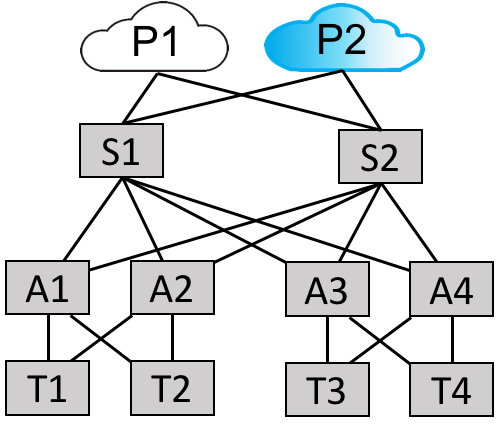
\includegraphics[width=.7\columnwidth]{figures/topology-con}
  \end{minipage}%
  %
  \begin{minipage}[t]{.4\linewidth}
    \hdr{Abstract Topology}{}
    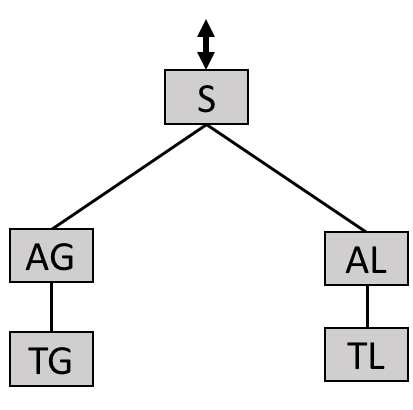
\includegraphics[width=.57\columnwidth]{figures/topology-abs}
  \end{minipage}%

  \vspace{2em}
  \begin{minipage}[t]{.6\linewidth}
    \hdr{Concrete Product Graph}{}
    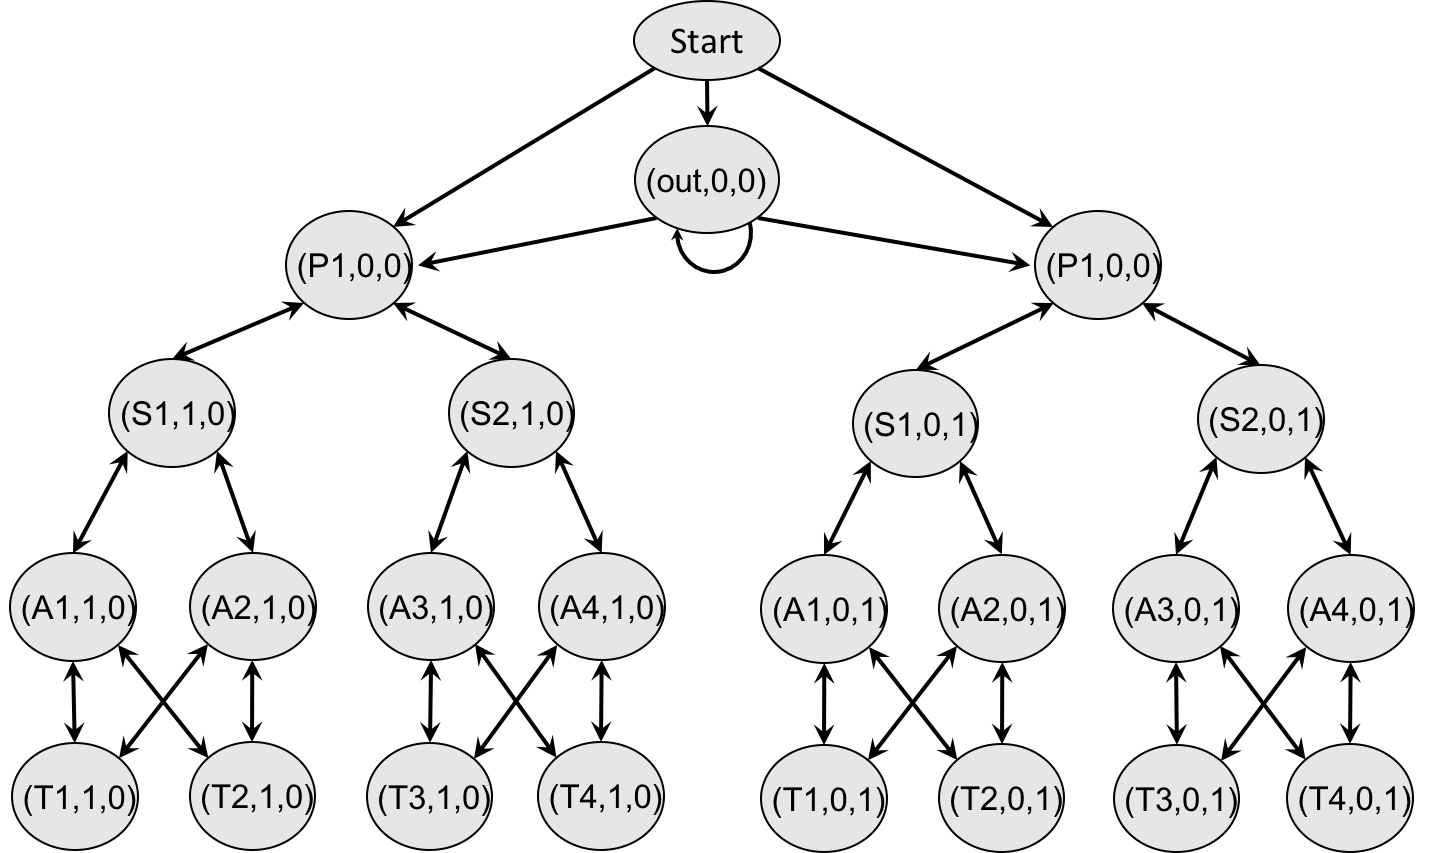
\includegraphics[width=.9\columnwidth]{figures/pg-con}
  \end{minipage}%
  \begin{minipage}[t]{.4\linewidth}
  \hdr{Abstract Product Graph}{}
    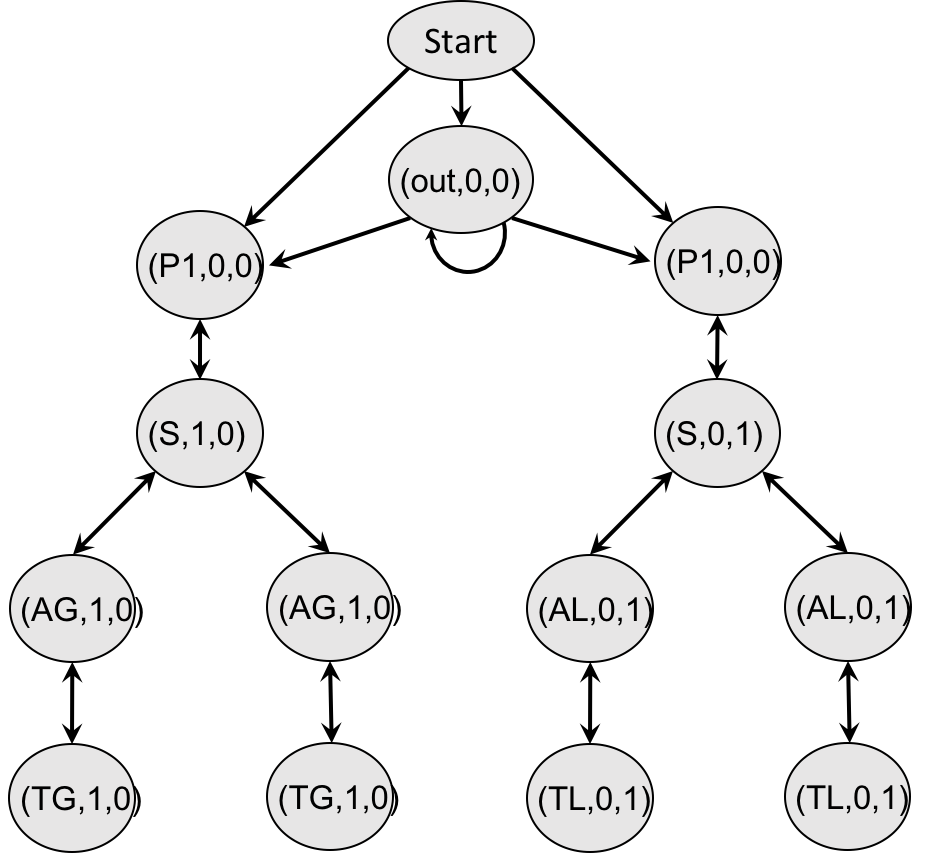
\includegraphics[width=.9\columnwidth]{figures/pg-abs}

  \end{minipage}%

  \hrulefill
  \vspace*{.4em}%

  \caption{Product graph construction for policy $true \Path \Exit(\text{Peer1} \Prefer \text{Peer2})$.}
  \label{fig:example-compilation}
  %\vspace{-1em}
\end{figure*}


\subsection{Compilation to configurations}

The translation from the Product Graph to per-device configurations that run the distributed BGP protocol involves several ideas. 

\para{Route filtering}

The first idea is to tag every protocol message with a BGP community value that relays the state of each automaton when advertising a route to a neighbor. Routers can then allow route advertisements that correspond to an edge in the Product Graph (\IE, from a neighbor with the correct state) and block those that don't. This ensures that any path computed by BGP will be a valid path in the Product Graph, and thus is allowed by the policy. For example, in the concrete Product Graph in figure~\ref{fig:example-compilation}, router $S1$ will allow a route advertisement from its neighbor $P1$ and also from neighbor $P2$. If it uses neighbor $P1$, then it will add the tag $(1,0)$ before informing its neighbors about its route. On the other hand, if it uses neighbor $P2$, then it will add the tag $(0,1)$ before informing its neighbors about the route.
%
However, letting BGP find some allowed path is not enough. \sysname must ensure BGP always computes the \emph{best} path according to the user's preferences, even when failures occur. 


\para{Preference Search}
The second idea is to totally order advertisements each router might receive from neighbors in the Product Graph by preference. For example, to satisfy the policy that leaving through $\sf{P1}$ is preferred to leaving through $\sf{P2}$, router $S1$ should prefer a route it hears from $P1$ over one from $P2$. Similarly, router $A1$ should prefer routes tagged with $(1,0)$ over those tagged with $(0,1)$.

In general, because BGP is distributed, each router does not have a full view of the entire network when choosing which path to use. Because finding a collection of preferences to ensure correct end-to-end behavior for all failures is a hard problem, Propane introduced a conservative, yet effective algorithm for determining route preferences based on the following observation about the structure of the Product Graph:

\begin{defn}
Let $m \geq_{rank} n$ be a relation over Product Graph vertices that holds iff $P(n) = \emptyset$ or $\min P(m) \geq \min P(n)$. Intuitively $m \geq_{rank} n$ means that paths ending at PGIR node $m$ are no better (higher rank) than paths ending at $n$.
%
\end{defn}
\noindent
%

\begin{defn}
The product graph can be viewed as a labelled transition system by pushing the topology location from each directed edge's target node onto the edge. That is, $m\overset{l}{\rightarrow}n$ if edge $(m,n) \in E'$ and $\tilde{n} = l$. 
\end{defn}

For example, in concrete product graph we would have the transition $(S1,1,0)\overset{A2}{\rightarrow}(A2,1,0)$

\begin{defn}
We write $m \leq m'$ if the subgraph reachable from $m$ and $m'$ respectively form a simulation relation with respect to the $\geq_{rank}$ relation on node rankings.
\end{defn}

We can assign BGP local preferences for the policy in the following way: Check if each router has a total order with respect to the simulation relation ($\leq$) for its corresponding Product Graph nodes. If so, then simply sort the nodes and prefer advertisements from peers of node $m$ over those of node $m'$ if $m' \leq m$.
 
For example, in the concrete product graph we have $(S1,0,1) \leq (S1,1,0)$ since nodes on the left side of the product graph can always match transitions made on the right hand side while always maintaining a node ranking that is at least as good as that on the right hand side (since they match the preferred rank 1 automaton). This relation does not hold the other way around. Therefore, advertisements received at $S1$ in state $(1,0)$ must be preferred to those received in state $(0,1)$. 

Notice also that in the abstract product graph, node $(S,0,1) \leq (S,1,0)$. This leads us the the following observation:

\begin{lem}
\label{lem:preference}
$m \leq m'$ in the concrete product graph iff $f_{pg}(m) \leq f_{pg}(m')$ in the abstract product graph under the lifted graph homomorphism $f_{pg}$.
\end{lem}

Lemma~\ref{lem:preference} gives us reason to believe that we can perform compilation over the abstract product graph and ensure that the inferred device-level preferences will be correct when instantiating the template with a concrete network.


\newcommand{\highlight}[1]{%
  \colorbox{red!50}{$\displaystyle#1$}}
\newcommand{\Router}[1]{\KW{Router} #1:}
\newcommand{\REGEX}[1]{\texttt{regex}(#1)}
\newcommand{\PEER}{\texttt{peer}}
\newcommand{\PREFIX}{\texttt{prefix}}
\newcommand{\IF}{\texttt{if}}
\newcommand{\THEN}{\texttt{then}}
\newcommand{\COMM}{\texttt{comm}}
\newcommand{\MED}{\texttt{MED}}
\newcommand{\Arrow}{\ensuremath{\leftarrow}}

\para{BGP configurations}

\begin{figure*}[t!]
  \begin{minipage}[t]{.54\linewidth}
    \hdr{Concrete Configuration}{}
    \begin{code}
      \Router{S1, S2}
        Match[100] \PREFIX=GP1, \PEER=*
          \PEER \Arrow *
        Match[100] \PREFIX=GP2, \PEER=*
          \PEER \Arrow *
        ...
        Match[100] \PREFIX=LP1, \PEER=\{AG1, ..., AL1, ...\}
          \PEER \Arrow \{AG1, ..., AL1, ...\}
        Match[100] \PREFIX=LP2, \PEER=\{AG1, ..., AL1, ...\}
          \PEER \Arrow \{AG1, ..., AL1, ...\}
        ...
        Match[110] \PREFIX=0.0.0.0/[0..32], \PEER=P1, 
          \PEER \Arrow *, \COMM \Arrow (1,0)
        Match[100] \PREFIX=0.0.0.0/[0..32], \PEER=P2, 
          \PEER \Arrow *, \COMM \Arrow (0,1)
        ...
      \end{code}
  \end{minipage}
  %
  \begin{minipage}[t]{.4\linewidth}
    \hdr{Template Configuration}{}
    \begin{code}
      \Router{S}
        Match[100] \PREFIX=\$GP, \PEER=*
          \PEER \Arrow *
        Match[100] \PREFIX=\$LP, \PEER=\{AG, AL\}
          \PEER \Arrow \{AG, AL\}
        Match[110] 0.0.0.0/[0..32], \PEER=P1, 
          \PEER \Arrow *, \COMM \Arrow (1,0)
        Match[100] 0.0.0.0/[0..32], \PEER=P2, 
          \PEER \Arrow *, \COMM \Arrow (0,1)
        ...
      \end{code}
  \end{minipage}%

  \hrulefill
  \vspace*{.4em}%

  \caption{Spine configurations for concrete and abstract policies. \ryan{TODO: this would look good in powerpoint and by connecting related components}}
  \label{fig:bgp-configs}
\end{figure*}

By combining the tagging, filtering and preference mechanisms, we can generate safe BGP configurations. In general, configurations are generated by combining the per-prefix configurations in the same order specified in the policy. Figure~\ref{fig:bgp-configs} shows part of the configuration for the spine routers for the concrete and abstract policies. 

The spine switches have a default rule for the prefix $0.0.0.0/[0..32]$ that will match advertisements from peer $P1$ and $P2$. The match for $P1$ is preferred since it has a higher BGP local-preference attribtue (110). If an advertisement from $P1$ is available the spine attaches the community tag $(1,0)$ and advertises the route to all its peers. If only an advertisement from the backup $P2$ is available, then it attaches the tag $(0,1)$ and advertises this to all peers instead. 

In the template configuration, it will have additional policy for the local and global prefixes. It will match any global prefix from any peer and re-advertise the route to all of its peers. For any local prefix it will allow an advertisement from any internal peer, and re-advertise the route to all other internal peers. The concrete configurations will have a similar configuration for each local and global prefix.


\subsection{Compilation Correctness}

\begin{easylist}[itemize]
& First show how to compile to the Product Graph, and from there to the ABGP
& Next define the concretization & subst. functions for translating the abstract policy
   into the concrete policy, using the ABGP example for reference
& Give abstraction theorem: commuting of concretization and compilation
\end{easylist}

\subsection{Incrementality}

Suppose that we want to expand the concrete datacenter by adding an additional tor router in the TG role. Per the network routing policy, this new ToR router will advertise its own owned prefix. Because the new topology matches the abstraction, the compiled templates will remain the same. However, in the spine router configurations, the match on the global prefix template variable \$GP will be expanded to include the new prefix owned by the ToR. In other words, the concrete configurations obtained after substitution will include an additional match on the new prefix. Unfortunately, this means a small change to the topology can result in many configurations far from the change needing to change too.

The key observation is that the template variables tell us exactly where change can happen. For example, the only way in which the spine routers depend on anything nonlocal is in the prefix template variables. Instead, we replace each match on a template variable (\EG, matching \$GP) with a test on a new community tag that we associate with each template variable. So long as we ensure that routers always add the appropriate tags to the prefixes they originate, then the policies will be equivalent.

Specifically, this ensures that each router has a template that has no dependency on any other non-adjacent router. If we make a change to the concrete network that matches the abstraction, then the templates do not change, and thus only configurations adjacent to the changes must also change. 




%=====================================================
%
%
%  **Abstractions**
%
%
%=====================================================


\section{Abstract Analysis}
\label{sec:analysis}

In the previous section we saw that \sysname can synthesize correct device configurations by operating directly over the abstract representation. However, in practice operators would often like to reason about other properties about their network. In this section we present an analysis that operates over the network abstraction to find a lower bound on the number of disjoint paths between pairs of concrete nodes. Answering questions about the number of disjoint paths allows operators to reason about many useful network properties such as reachability (\IE, is there at least one path) and fault tolerance (\EG, how many failures will disconnect certain routers). An important point is that the analysis takes place over the structure of the product graph, and so takes both the topology and routing policy into account.


\newcommand{\inference}[4]{
    \node[draw, anchor=west] at (#1 + .4, 1.25) {#3};
    \node at (#1 + .34, .6) {$e_1$};
    \node at (#1 + .34, 1.9) {$e_2$};
    \node at (#1, -.8) {#2};
    \node at (#1, 3.3) {#4};
    \draw [] (#1, 2.5) circle [radius=0.45] node {$m$};
    \draw [] (#1, 0) circle [radius=0.45] node {$n$};
    \draw [] (#1, .45) -- (#1, 2.05);
}

\begin{figure*}[t!]
  \begin{minipage}[t]{.5\linewidth}%
  \begin{tikzpicture}
    \inference{0}{L$(j,k)$}{$\vDash e_1 > 0$}{S$(min(j*k,e_1),1)$}
    \inference{5}{A$(j,k)$}{$e_2 > 0$}{A$(1,min(j,e2))$}
    \inference{10}{L$(j,k)$}{$e_1=n$}{A$(min(j*k,n),1)$}
    \inference{15}{L$(j,k)$}{$e_1=n$}{A$(1,j)$}
  \end{tikzpicture}
  \end{minipage}

  %
  \vspace*{3em}
  %
  \begin{minipage}[t]{.5\linewidth}%
  \begin{tikzpicture}
    \inference{0}{L$(j,k)$}{$e_1 > 0$, $e_2 > 0$}{S$(min(j*k,n-\dfrac{(m-j)*e_1}{e_2}),1)$}
    \inference{10}{L$(j,k)$ ~~~ L$(j- m ~\text{mod}~ \big(\dfrac{n}{e_1}\big),1)$}{$e_1 > 0$, $e_2 > 0$}{}
  \end{tikzpicture}
  \end{minipage}

  \vspace*{1em}
  \hrule
  \vspace*{1em}
  \caption{Abstract k-disjoint path analysis inference rules.}
  \label{fig:abstract-analysis}
  %\vspace{-1em}
\end{figure*}


\subsection{Abstract k-disjoint paths}
\label{sec:property-checking}

In order to infer bounds on the number of disjoint paths between nodes we use information about the structure of the underlying concrete topologies encoded in the abstraction pod structure and node + edge multiplicity constraints.

The idea is to maintain, for each role in the abstract product graph, facts learned about the number of disjoint paths to some number of concrete routers in that role from a given source location. More specifically, we maintain facts of the form:
%
\[ \begin{array}{c}
  L_{X_1}, \ldots, L_{X_n}(j,k) 
\end{array} \]
\noindent
%
Each label $L \in \{S,A\}$ is either $S$, which stands for ``some" or is $A$, which stands for ``all". There is one label in the nesting for each pod scope in the network abstraction hierarchy. So for a given node, $L_{X_1}$ would correspond to the outermost pod scope, while $L_{X_n}$ would correspond the the node's label.

Semantically, $L_{X_1}, \ldots, L_{X_n}(j,k)$ means that starting from some concrete router in the abstract source, for ``some"/``all" scopes $X_1$, $L_{X_2}, \ldots, L_{X_n}(j,k)$ holds. The base case $L_{X_n}(j,k)$ means that for ``some"/``all" groups of size $j$ concrete routers, there are $k$ disjoint paths to each such that all $j*k$ paths are disjoint

\begin{figure}
  \begin{center}
    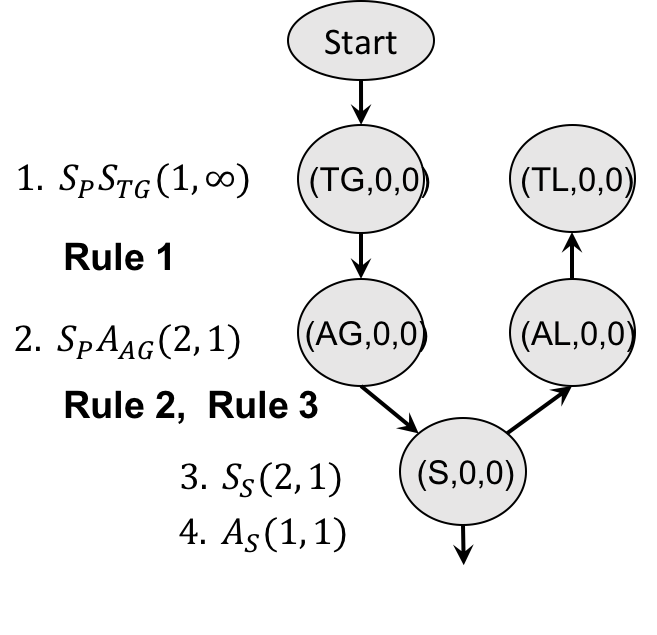
\includegraphics[width=.66\columnwidth]{figures/analysis}
  \end{center}
  \caption{Abstract disjoint path analysis with valleyfree routing for global prefixes. \label{fig:compilation-times}}
  \vspace{-1em}
\end{figure}

For example, a fact of the form: $A_P, S_{TL}(2,4)$ means that for all pods P, there is some group of size 2 concrete routers in role TL such that they each have 4 disjoint to them from the source and all 8 paths are disjoint. 

%suppose we want to compute the number of disjoint paths from the local ToR role $(TL,0,0)$ for  
\ryan{TODO: probably need a new image for local prefixes?}

%=====================================================
%
%
%  **Implementation**
%
%
%=====================================================


\section{Implementation}
\label{sec:implementation}

The \sysname compiler is implemented in approximately 9500 lines of F\# code. The compiler accepts both concrete and abstract topologies and will generate router configurations for open-source Quagga routers. Operators can specify their required fault tolerance level for aggregation safety. The abstract safety analysis uses Z3Opt \ryan{reference} to minimize variables subject to the annotated constraints. Since the analysis typically calls Z3 with many times with relatively simple optimization problems, we use a timeout of 200ms. 

The compiler performs the following to improve its performance.

\para{Z3 memoization}

Although the k-disjoint path analysis takes place over the Product Graph representation, which may differ from the topology (e.g., for non-shortest paths routing), each application of the inference rules from figure~\ref{fig:abstract-analysis} depends only on the topology. Therefore, we lazily apply the rules and cache the satisfiability and minimization calls to Z3 after their first use. Doing this significantly speeds up the failure safety analysis. Furthermore, the cached results can be shared across different prefixes, each of which may have a unique Product graph representation. In practice, this means that after performing the abstract analysis for one prefix, the analysis becomes essentially "free" for any subsequent prefixes.

\para{Fast Substitution}

Substitution after compiling a policy abstractly can be expensive since each router must substitute all template variables for each of its connected peers. In practice, because many routers often share the same concrete peers, memoizing the substitution function greatly improves performance.


%=====================================================
%
%
%  **Evaluation**
%
%
%=====================================================


\section{Evaluation}
\label{sec:evaluation}

We apply \sysname on policies for backbone and datacenter networks. We aim to evaluate the expressiveness of our abstract multiplicity annotations, the precision of the abstract disjoint-path analysis, and the compilation time of \sysname both with abstraction and without.

\subsection{Analysis precision}

\begin{figure}[t!]
  \begin{center}
      \begin{tabular}{| l | c | c | c |}
      \hline
      \textbf{Topology} & \textbf{Fixed} & \textbf{Reachable} & \textbf{K-paths} \\ \hline
      Google Fattree & & \cmark & \cmark  \\ \hline
      Facebook Fattree & & \cmark & \cmark \\ \hline
      Microsoft Fattree & & & \\ \hline
      F10 Fattree & & \cmark & \cmark \\ \hline
      BCube & $k$ & \cmark & \xmark \\ \hline
      DCell & $k$ & \cmark & \xmark \\ \hline
         %& HCN & $h$ & \cmark & \xmark \\
      Butterfly & $n$ & \cmark & \cmark \\ \hline
      Hypercube & $N$ & \cmark & \cmark \\ \hline
      HyperX & $L$ & \cmark & \cmark \\ \hline
      \end{tabular}
  \end{center}
  \caption{Abstract Analysis Precision.}
  \label{fig:analysis-precision}
\end{figure}

%\begin{figure}[t!]
%  \begin{center}
%      \begin{tabular}{| l l | c | c | c |}
%      \hline
%      \textbf{Topology} & \textbf{Variant} & \textbf{Fixed} & \textbf{Reachable} & \textbf{K-paths} \\ \hline
%      Fattree
%         & Google &  & \cmark & \cmark  \\
%         & Facebook &  & \cmark & \cmark \\
%         & F10 &  & \cmark & \cmark \\ \hline
%      Recursive
%         & BCube & $k$ & \cmark & \xmark \\
%         & DCell & $k$ & \cmark & \xmark \\ \hline
%         %& HCN & $h$ & \cmark & \xmark \\
%      Hypercube
%         & Standard & $N$ & \cmark & \cmark \\
%         & HyperX & $L$ & \cmark & \cmark \\ \hline
%      Random \footnote{foo}
%         & Scafida &  & ??? & ??? \\
%         & JellyFish &  & ??? & ??? \\
%      \hline
%      \end{tabular}
%  \end{center}
%  \caption{Abstract Analysis Precision.}
%  \label{fig:analysis-precision}
%\end{figure}

We evaluate the expressiveness and precision of our abstract analysis on a range of different network topologies found in both the network literature and production. For each topology in figure~\ref{fig:analysis-precision} we define a suitable abstraction. Since many topologies have tunable parameters (e.g., the recursion depth $k$ for the DCell topology), we list all such parameters that are fixed for our abstraction. We implement a shortest path routing policy over the topology and record the precision of the abstract analysis in terms of whether or not it is able to accurately prove reachability and/or the correct number of disjoint paths between all pairs of nodes.

\para{Fat Tree Topologies}

The Fat Tree topology is one of the most widely used datacenter topologies. We look at the precision of our analysis on three variants of the Fat Tree~\cite{foo} topology used in practice: the Google Fat Tree, the Facebook Fat Tree, and the F10 fault tolerant Fat Tree. For each Fat Tree variant, we use a tiered abstraction similar to that in our previous example \ryan{Reference}. Each Fat Tree topology is parameterized over the number of pods $k$, which can be scaled up in the abstraction to allow for expansion. For all Fat Tree variants, the analysis is precise enough to determine the exact number of disjoint paths between all pairs of concrete routers.

\para{Recursive Topologies}

We also model several recursive topologies using our abstractions. These include the BCube and DCell topologies. Each topology includes a recursion depth parameter ($k$), which we must fix. For a recursive topology with depth $d$, we model it as an abstract topology consisting of abstract nodes for each of the depth $d-1$ subcomponents. This allows for safe expansion within a subcomponent, but not from increasing the recursion depth. The analysis is able to accurately determine reachability (i.e., at least 1 disjoint path) for each recursive topology, but is overly conservative in determining k-disjoint paths. For the BCube topology, it is able to to determine the correct number of disjoint paths between some pairs of nodes, but not all.

\para{Hypercube Topologies}

Hypercube variants can be used as an alternative to Clos-style topologies for networks with high-radix (port density) switches. The HyperX topology can be viewed as a generalization of the hypercube, which includes parameters $L$ for the lattice dimension of the network, $S_i$ for the node multiplicity of each dimension $i$, $K_i$ for the bandwidth of links for each dimension, and $T$ for the number of terminal nodes (servers) connected to each router. For a fixed number of dimensions $L$, we abstract each full mesh of $S_L$ nodes into its own abstract node. The $S_{x-1}$ groups of abstract nodes can be captured using pods of the abstract $S_x$ nodes.

%\para{Random Network Topologies}
%
%Random networks such as Scafida and Jellyfish have seen a great deal of interest in academia. These topologies were designed with an eye towards incremental expansion and are based on probabilistic arguments of bisection bandwidth in random regular graphs. However, because the topologies are created randomly, there are no hard guarantees on the connectivity between different routers. We can trivially represent these networks using a \emph{one big switch} abstraction for the entire network.


\subsection{Compilation time}

\begin{figure}
  \subcaptionbox{Datacenter}
    {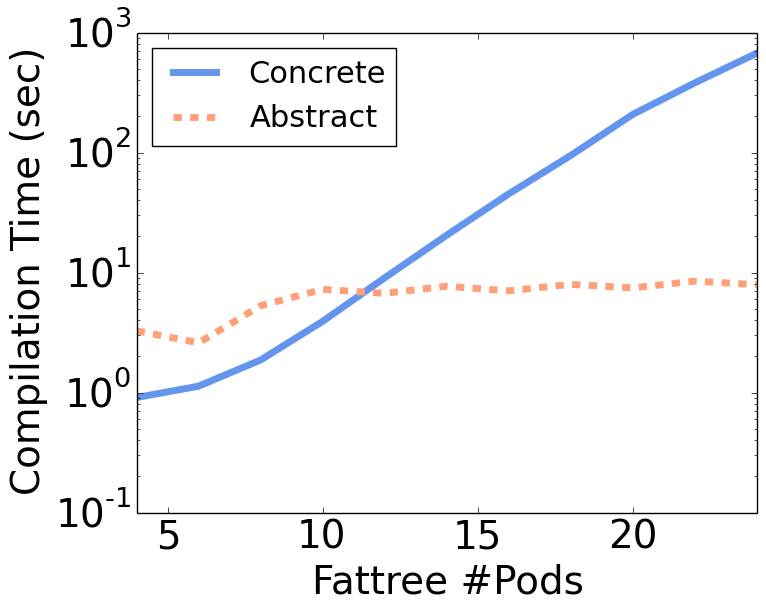
\includegraphics[width=.49\columnwidth]{figures/Fattree-time.png}}
  \subcaptionbox{Backbone}
    {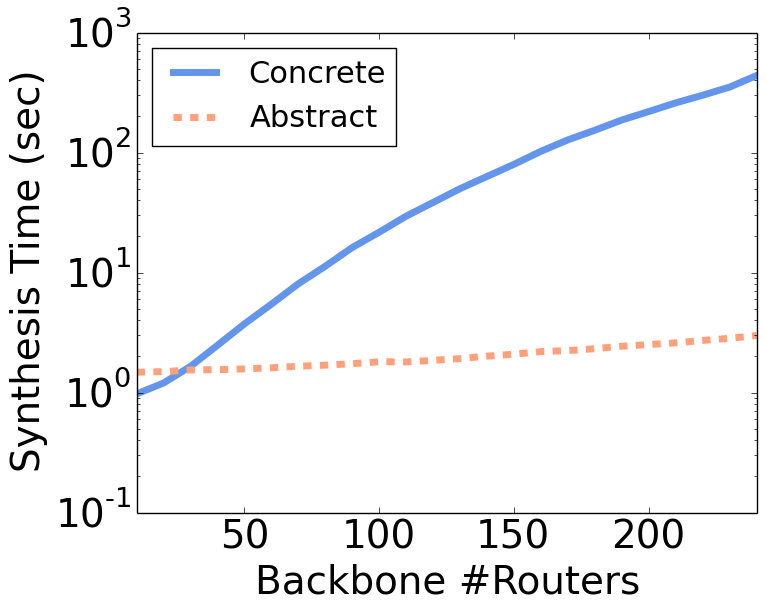
\includegraphics[width=.49\columnwidth]{figures/backbone-time.png}} \\
  \caption{Concrete vs. Abstract Compilation Time. \label{fig:compilation-times}}
  \vspace{-1em}
\end{figure}

\begin{figure}[t!]
  \subcaptionbox{Datacenter}
    {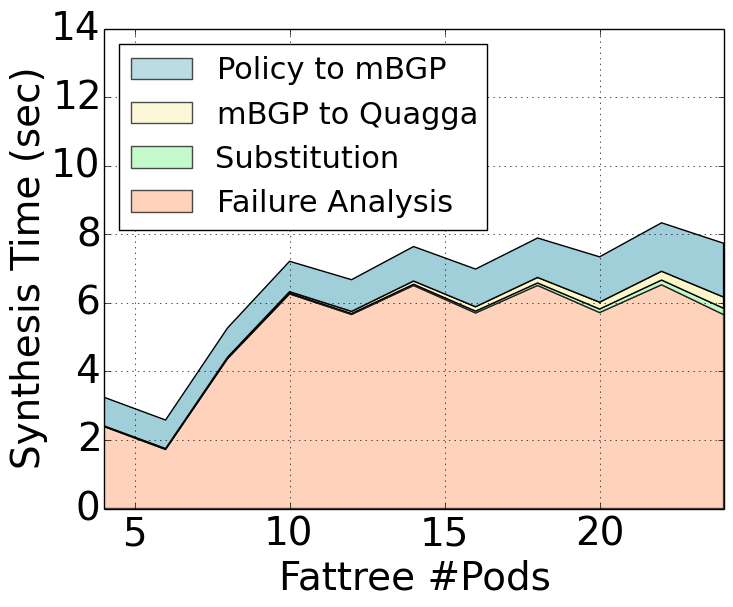
\includegraphics[width=.49\columnwidth]{figures/Fattree-analysis-time.png}}
  \subcaptionbox{Backbone}
    {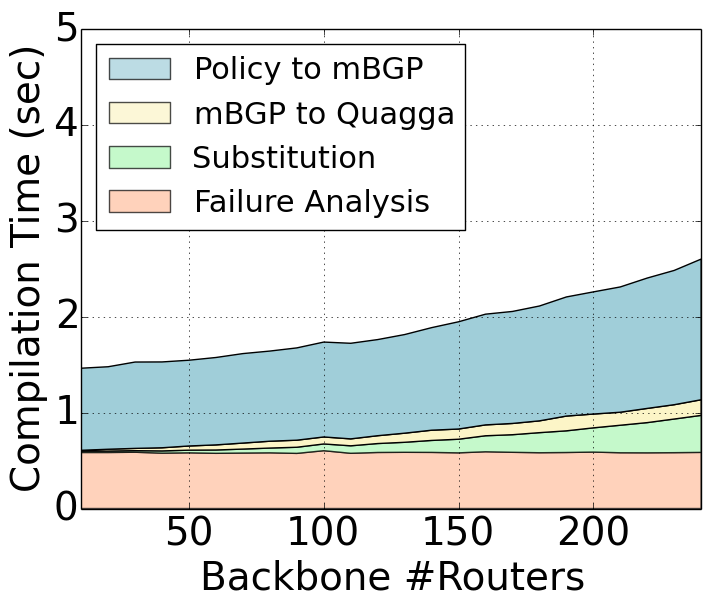
\includegraphics[width=.49\columnwidth]{figures/backbone-analysis-time.png}} \\
  \caption{Abstract Compilation Time by Phase. \label{fig:abstract-breakdown}}
  \vspace{-1em}
\end{figure}

Using abstraction allows us to naturally scale network synthesis in \sysname. We evaluate compilation time in \sysname both with and without abstraction using routing policy for backbone and datacenter networks inspired by configurations obtained from a large cloud provider.

\para{Routing Policy}

Routers in the datacenter network run BGP using private AS numbers and peer with each other and with the backbone network over eBGP. The routers aggregate some prefix blocks when announcing them to the backbone network, and they keep some prefixes internal. The policy also ensures bogons and private address space from external neighbors is dropped. The data center prefers that traffic leave through certain peers over others and ensures that transit traffic between peers is never allowed in the datacenter.

The backbone network classifies external neighbors into several different categories based on commercial relationship and prefers paths through them in order. Similar to the datacenter, it prevents bogons and private address space from external neighbors, drops transit traffic between certain peers but not through others, and aggregates internal prefixes at the border of the network.

\para{Network Topology}

For both networks, we use the same routing policy but scale the size of the underlying topology. For the datacenter networks, we use a standard Fat Tree topology and scale the size of the topology according the the number of pods $k$, starting with 4 pods and ending with 24 pods. The abstract topology uses a single abstract node for each tier of the datacenter, an additional abstract node for tier 0 to separate local and global prefixes, as well as a single abstract node for each group of equivalent eBGP neighbor.

For the backbone networks, we split the network into two parts: a collection of border routers and a fully-connected internal core. We scale the backbone networks from 10 to 250 routers. The abstract topology uses a single abstract node for the network border routers and another abstract node for the network core. Backbone eBGP-speaking peers are grouped into abstract nodes based on their commercial relationship to the current AS (e.g., customer, provider, peer).

\para{Results}

Figure~\ref{fig:compilation-times} shows compilation time for the same policies for both the abstract and concrete versions of the policies described above. All experiments are run on an 8 core, 2.4 GHz Intel i7 processor Mac with 8GB of Ram.

For both the datacenter and backbone networks, the abstract compilation starts off slightly slower than concrete compilation for small topologies due to the overhead of the abstract k-disjoint path analysis for aggregation black-hole safety. However, as the size of the topology increases, abstract compilation becomes orders of magnitude faster than concrete compilation. In all cases for both networks, abstract compilation takes less than 10 seconds to complete.

Figure~\ref{fig:abstract-breakdown} shows the relative time taken by each phase of abstract compilation. Notably, the abstract analysis takes the majority of the time, however the analysis does not depend on the number of concrete nodes in the network, and thus is largely a fixed cost. In particular, the number of calls to Z3 remains constant the across topology size. The seesaw behavior for the data center networks results from differences in time taken by Z3 to minimize the same constraints with different parameters.




%=====================================================
%
%
%  **Related Work**
%
%
%=====================================================

\section{Related Work}
\label{sec:related}

\begin{easylist}[itemize]
& Topologies: DCell, BCube, Fattree, ...
& Topology Abstraction: Condor
& Memory Shape Analysis: Sagiv, others
& Configuration automation
& Configuration analysis
& Configuration synthesis
\end{easylist}

%Our work draws on four threads of prior work.%

%\para{Topology abstraction}%

%\para{Topology design}%

%\para{Configuration automation}
%Many practitioners use configuration templates~\cite{hatch,thwack}, to ensure certain kinds of consistency across similar devices. In addition, configuration languages such as RPSL~\cite{RFC2622}, Yang~\cite{RFC6020}, and Netconf~\cite{RFC6241} allow operators to express routing policy in a vendor-neutral way.
%However, all of these solutions remain low-level, for example, requiring operators to specify exact local preferences. Unlike \sysname, there is no guarantee that these low-level configurations satisfy the original, high-level intent.%

%\para{Configuration analysis}
%The notion that configuring network devices is difficult and error-prone is not new.
%In the past, researchers have tried to tackle this problem by analyzing existing
%router configurations~\cite{feamster+:rcc,ipassure,batfish,bagpipe,arc} and reporting errors or inconsistencies when they are detected.
%Our research is complementary to these analysis
%efforts.  We hope to eliminate bugs by using higher-level
%languages and a ``correct-by-construction''
%methodology. Writing configurations at a high level of abstraction simplifies policy implementation and prevents a whole host of low-level errors.%

%\para{Configuration synthesis}
%ConfigAssure~\cite{narain:lisa05,narain+:configassure}
%is another system designed to
%help users define and debug low-level router
%configurations.  Inputs to
%ConfigAssure include a \emph{configuration database}, which contains a
%collection of tuples over constants and configuration variables, and a
%\emph{requirement}, which is a set of constraints.
%%
%The authors use a combination of logic programming and
%SAT solving to find concrete values for configuration variables.
%ConfigAssure handles configuration for a wide range of protocols and many
%different concerns.  In contrast, the scope of \sysname is much
%narrower.  In return, \sysname offers compact, higher-level
%abstractions customized for our domain, such as regular paths, as well
%as domain-specific analyses customized to those abstractions, such as
%our failure safety analysis.  The implementation technology is also
%entirely different, as we define algorithms over automata and graphs
%as opposed to using logic programming and SAT-based model-finding.



%=====================================================
%
%
%  **Conclusions**
%
%
%=====================================================

\section{Conclusions}
\label{sec:conclusions}



\para{Acknowledgments}




%=====================================================
%
%
%  **Bibliography**
%
%
%=====================================================

\balance

\bibliographystyle{abbrv}
\bibliography{references}


%=====================================================
%
%
%  **Appendix**
%
%
%=====================================================

\appendix

\begin{figure*}[t]\small
  \begin{minipage}[t]{.45\linewidth}
  \hdr{Syntax}{}
  \vspace*{-1\baselineskip}
  %
  \[ \begin{array}{rclr}
    \hline%

     pol     &::=& p_1, \dots, p_n & \textit{policies} \\
     p       &::=& t \hspace{.3em} \Path \hspace{.3em} r_1 \Prefer \dots \Prefer r_m \BNFALT cc & \textit{constraints} \\
     x       &::=& d.d.d.d/d & \textit{prefix} \\
     t       &::=& \True & \textit{true} \\
         &\BNFALT& \neg t & \textit{negation} \\
         &\BNFALT& t_1 \vee t_2 & \textit{disjunction} \\
         &\BNFALT& t_1 \wedge t_2 & \textit{conjunction} \\
         &\BNFALT& \textit{prefix} = x & \textit{prefix test} \\
     r       &::=& l & \textit{location} \\
         &\BNFALT& \emptyset & \textit{empty set} \\
         &\BNFALT& \In & \textit{internal loc} \\
         &\BNFALT& \Out & \textit{external loc} \\
         &\BNFALT& r_1 \cup r_2 & \textit{union} \\
         &\BNFALT& r_1 \cap r_2 & \textit{intersection} \\
         &\BNFALT& r_1 \cdot r_2 & \textit{concatenation} \\
         &\BNFALT& \NOT r & \textit{path negation} \\
         &\BNFALT& r^* & \textit{iteration} \\
     cc     &::=& agg(x, r_1 \rightarrow r_2)  & \textit{control constraints} \\
  \end{array} \]%

  \end{minipage}
  %
  ~~
  \vrule
  ~~
  %
  \begin{minipage}[t]{.5\linewidth}\small
  \hdr{Propane Expansions}{}
  \vspace*{-1\baselineskip}
  %
  \[\begin{array}{rcl}
    \hline
    \Any               & = & \Sigma^* \\
    \None              & = & \emptyset \\
    \Internal          & = & \In^+ \\
    \Always(X)         & = & X^* \\
    \Never(X)          & = & (!X)^* \\
    \Through(X)        & = & \Sigma^* \cdot X \cdot \Sigma^* \\
    \Eventually(X)     & = & \Out^* \cdot (X \cap \Out) \cdot \Out^* \cdot \In^+ \cdot \Out^* \\
    \Already(X)        & = & \Out^* \cdot \In^+ \cdot \Out^* \cdot (X \cap \Out) \cdot \Out^* \\
    \End(X)            & = & \Sigma^* \cdot X \\
    \Start(X)          & = & X \cdot \Sigma^* \\
    \Enter(X)          & = & \Sigma^* \cdot \Out \cdot (X \cap \In) \cdot \Sigma^* ~ \cup \\
                       &   & \Sigma^* \cdot (X \cap \Out) \cdot \In \cdot \Sigma^* \\
    \Exit(X)           & = & \Sigma^* \cdot \In \cdot (X \cap \Out) \cdot \Sigma^* ~ \cup \\
                       &   & \Sigma^* \cdot (X \cap \In) \cdot \Out \cdot \Sigma^* \\
    \LinkKW(X,Y)       & = & \Sigma^* \cdot X \cdot Y \cdot \Sigma^* \\
    \PathKW(\vec{X})   & = & \Sigma^* \cdot X_1 \dots X_n \cdot \Sigma^* \\
    \Novalley(\vec{X}) & = & \NOT\PathKW(X_2,X_1,X_2) ~ \cap \dots \cap \\
                       &   & \NOT\PathKW(X_n,X_{n-1},X_n) \\
  \end{array} \]%

  \end{minipage}%

  \hrulefill%

  \caption{Regular Intermediate Representation (RIR) syntax (left), and
           Propane language expansions (right).}
  \label{fig:rir-syntax}
  %\vspace{-1em}
\end{figure*}%





\end{document}
